\documentclass[12pt,a4paper,twoside]{article}
    \special{papersize=210mm,297mm}
    
    \usepackage[a4paper,includeheadfoot,margin=2.54cm]{geometry}
    \usepackage{pdflscape}
    \usepackage{hyperref}
    \usepackage{natbib}

    \usepackage[utf8]{inputenc}
    \usepackage{graphicx}
    \usepackage[danish]{babel}

    \usepackage[familydefault,regular]{Chivo}
    \usepackage[T1]{fontenc}

    \usepackage{lastpage}
    \usepackage{fancyhdr}
    \usepackage{xcolor}
    \usepackage{mathtools}
    \usepackage{amsmath}
    \usepackage{gensymb}
    %Plotning af 
    \usepackage{pgfplots}
    \usepackage{pdfpages}
    %\pgfplotset{width=10cm,compat=1.9}
    \usepackage{multirow}     
    %\usepackage{tabularx}
    \usepackage{booktabs}% http://ctan.org/pkg/booktabs
    \newcommand{\tabitem}{~~\llap{\textbullet}~~}

    \newcommand{\todo}[1]{\textcolor{red}{TODO: #1}\PackageWarning{TODO:}{#1!}}
                 
    \pagestyle{fancy} 
    \fancyhf{}
    \fancyhead[LE,RO]{Et kig på IBI i privaten}
    \fancyhead[RE,LO]{\rightmark}
    \fancyfoot[CE,CO]{Michael Torp Kaalund, Hold: elsp4d18}
    \fancyfoot[LE,RO]{Side \thepage \hspace{1pt} af \pageref{LastPage}}
    \renewcommand{\headrulewidth}{1.5pt}
    \renewcommand{\footrulewidth}{1.5pt}
 
    %% Ny 
    \newcommand{\vdc}{V$_{\text{DC}}$ }
    \newcommand{\vac}{V$_{\text{AC}}$ }

    \title{Et kig på IBI i privaten}
    
    \author{Michael Torp Kaalund \thanks{Mange tak til min læreplads Intego A/S}}
    
    \begin{document}
  
    \begin{titlepage}
    \centering
    {\usefont{T1}{pag}{m}{b}\LARGE Den jydske håndværkerskole i Hadsten \par}
    \vspace{1cm}
    {\usefont{T1}{fvs}{m}{b}\Large Svendeprøve som elektriker \par}
    \vspace{1.5cm}
    {\huge\bfseries Et kig på IBI i privatboligen \par}
    \vspace{10cm}
    {\usefont{T1}{qzc}{m}{it} Michael Torp Kaalund, Intego A/S Randers afd. \par}
    {\usefont{T1}{qzc}{m}{it} Hold: elsp4d18 \par}
    \vfill
    {\bfseries \today\par}
\end{titlepage}


%    \begin{abstract}
%        TODO: Skrive omkring hvad projektet går ud på.
%    \end{abstract}

    %\cleardoublepage 



    \tableofcontents

    %\newpage
    
    %\section{Projektbeskrivelse}
\textbf{Dato:} \today \\
\textbf{Navn:} Michael Torp Kaalund\\
\textbf{Valg af moduler i uddannelsen:}
\begin{itemize}
    \item Modul 1.3 Automatiske anlæg i bygninger
    \item Modul 1.4 Intelligente bygningsinstallationer (centrale) og design af enkle brugerflader
    \item Modul 1.6 Design og styring af lys
    \item Modul 2.2 Styring og regulering af automatiske anlæg
\end{itemize}
\textbf{Moduler, der indgår i svendeprøven:}
\begin{itemize}
    \item Modul 1.3 Automatiske anlæg i bygninger
    \item Modul 1.4 Intelligente bygningsinstallationer (centrale) og design af enkle brugerflader
    \item Modul 2.2 Styring og regulering af automatiske anlæg
\end{itemize}
\textbf{Klasse:} elsp4d18

\begin{enumerate}
    \item \textbf{Angiv hvem der har ansvar for hvilke områder af projektet, hvis der arbejdes i en
    gruppe:}\\ Da jeg har valgt, at arbejde alene. Så det fulde ansvar er hos mig.
    \item \textbf{Problemstilling og formål med projektet:} \\ 
    Kunden ønsker at få et automatiseret drivhus styring. Som
    automatisk fylder vand i planteboksene fra hans regnvandsopsamling.
    Styringen skal kunne holde et konstant niveau i plantekasserne. \\
    Kunden får lavet en lysinstallation med IHC. 
    %Kunden har et ønske om, at få en lysstyring som både kan styre den IHC og
    %IKEA Trådfri / Philips HUE. 
    \\
    Kunden ønsker også, at ventilationsanlægget, skal kunne komme ind over styringen.
    Hvordan kan det være muligt, at lave kommunkation som kan over flere flader?
    % (f.eks IHC, IKEA Trådfri, ventilationsanlægget osv.)\newcounter{enumi_saved}

    \item \textbf{Indhold af projektet, herunder mulige tekniske løsningsmodeller} \\ 
    Med den tid som er tilrådighed ville det blive presset hvis der skulle laves og dokumenteres installationen og programmingerne af et helt hus, samt design af drivhus styringen. 
    Drivhus styring ville der blive lagt vægt på samt hvordan en intelligent bygningsinstallation kunne programmeres op.
    Det innovative del af projektet er automatisering af drivhuset i en privat bolig. Selv om der har fået et fremryk de seneste par år, med en smart lysstyring i bolig, så er det langt fra alle løsninger som er optimale i forhold til hvordan brugeren udnytter dette. 
    \\
    Vandstyringen til drivhusstyringen
    \begin{itemize}
        \item Siemens LOGO! 12/24RCE
        \item Siemens LOGO! Power 24V 2,5A
        \item Akvarie Pumpe
        \item 2 stk Vandniveau måler med 0 - 10V udgang, eller et potentiometer ( $5k\Omega$) og en serie modstand ($6,6k\Omega$) \footnote{Side 42 \cite{logo_sm} }
        \item Tavle med din skinne eller montage boks med din skinne.
        \item $3g1,5mm^2$ tilledning
        \item 3pol stikprop
        \item C6A automatsikring eller en B10A automatsikring.
        \item Sløjfeledning $1mm^2 - 2,5mm^2$
    \end{itemize}
    Eventuelle udstyr til lysstyring
    \begin{itemize}
        \item IHC controller
        \item IHC strømforsyning
        \item IHC 230V output relæ
%        \item IKEA Trådfri pære 3 stk
%        \item IKEA Trådfri tryk
%        \item IKEA Trådfri gateway
        \item WiFi Router inkl. switch
%        \item Raspberry PI 3 model B+
%        \item 5V 2,5A strømforsyning (usb lader)
%        \item Nilan Comform 300 ventilationsanlægget med CTS602
%        \item Nilan Connect 
        \item IHC input 24/3
        \item IHC output 24
        \item IHC Fugt sensor
    \end{itemize}

    \item \textbf{Beskrivelse af opgaver eller installationer, der kan demonstrere dine tekniske,
    håndværksmæssige og innovative færdigheder} \\ 
    Der ville opbygges en test opstilling af drivhusstyringen. Der ville blive lavet en tegning og en beregning af ventilationsanlægget, samt der ville beskrivelse hvordan styringen kan automatiseret. Der ville beskrivelses hvordan der ville kunne være en central styringen til lysinstallation.
 
    \item \textbf{Forslag til dokumentation for de valgte løsninger.}
    \begin{itemize}
        \item Brugervejledning.
        \item Tekniske tegninger.
        \item Relevante beregninger.
        \item Beskrivelse af love og regler som er gældene.
    \end{itemize}
    \item \textbf{Tidsstyring af projektet:}
    \begin{itemize}
        \item Den budgeteret tidsplan, ville blive opsat i Microsoft Excel eller i et lignene program.
        \item Der ville også blive lavet en realiseret tidsplan i samme format.
        \item Der ville blive lavet en status ved afslutning af arbejdsdagen.
    \end{itemize}
   
\end{enumerate}

    \section{Implementering}
    %    \subsection{Drivhus styring}

I kundens drivhus skal der dyrkes tomater og agurker som har fordel af en relativ luftfugtighed på 70\% - 80\%.
Da dette drivhus ikke er opvarmet, så bliver tomatplanterne udplantet omkring den 1. maj og agurk planterne i slutningen af maj.
Temperaturen i drivhus bør i dagstimerne være mellem 20$^\circ$C - 30$^\circ$C, og helst ikke meget over, da planterne ikke kan holde til varmen.

\subsubsection{Luftfugtighed}
Luftfugtighed fortæller hvor mange gram vand der er i en m$^3$ luft ved en given temperatur.
Hvis vi kigger på figure \ref{fig:luft_vanddamp}, så kan der ses at mængden af vand som luften kan optage er en konstant, men er afhængelige af temperaturen.
Det kan også ses at det ikke er en linære afhængelig af temperaturen.
Så tit ville man bruge relativ luftfugtighed (angivet som \%RF eller \%RH), som angiver luftfugtighed som en er procentsats. 
Da enheden bliver temperatur uafhængeligt og siger om hvor meget vand der i forhold til luften.

%Tomat i drivhus uden varme er fra omkring 1. maj
%Agurk i drivhus uden varme og som små planter i slutningen af maj til juni.

%Begge planter kan ikke klar temperature over 30 grader celcius.

%Luftfugtighed ønskes til at være omkring.

%Reduktion af Luftfugtighed kan ske via ventilation. \url{http://pure.au.dk/portal/files/42028244/743458.pdf}
%Luftfugtighed agurk: 2 g kg$^{-1}$ 
%Luftfugtighed tomat: 3 g kg$^{-1}$ 
%80 \% RH

%\url{https://www.havenyt.dk/spoergsmaal/drivhuset/12188.html}
%Tomater: 20 grader om dagen
%Agurk: 26 - 28 grader om dagen
%\url{https://voresvilla.dk/haven/drivhus-orangeri/undga-sygdomme-drivhuset/}
%Op til 4 liter vand om dagen.
%\url{http://old.gyproc.dk/files/Gyproc/Library/Handbook/DK/HB9%20-%204.5.2%20-%20Fugt%20i%20luft.pdf}
%\url{http://www.vitavia.dk/filarkiv/pdf/Vitavia_broc_2017_DK_low.pdf}

\begin{figure}[!h]
    \begin{center}
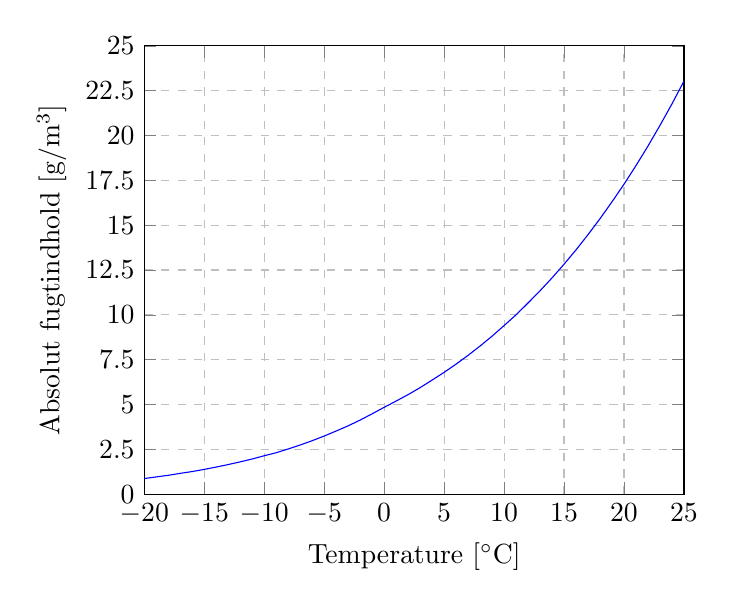
\begin{tikzpicture}
\begin{axis}[
    %title={Luft mættet med vanddamp},
    xlabel={Temperature [$^{\circ}$C]},
    ylabel={Absolut fugtindhold [g/m$^3$]},
    xmin=-20, xmax=25,
    ymin=0, ymax=25,
    xtick={-20, -15, -10, -5, 0, 5, 10, 15, 20, 25},
    ytick={0.0, 2.5, 5.0, 7.5, 10.0, 12.5, 15.0, 17.5, 20.0, 22.5, 25.0},
    %legend pos=north west,
    ymajorgrids=true,
    xmajorgrids=true,
    grid style=dashed,
]
\addplot[
    color=blue,
    mark=dot,
    ]
    coordinates {
        (-20,0.87)
        (-19,0.96)
        (-18,1.05)
        (-17,1.16)
        (-16,1.26)
        (-15,1.38)
        (-14,1.51)
        (-13,1.65)
        (-12,1.80)
        (-11,1.96)
        (-10,2.14)
        (-9,2.31)
        (-8,2.52)
        (-7,2.74)
        (-6,2.98)
        (-5,3.24)
        (-4,3.52)
        (-3,3.81)
        (-2,4.13)
        (-1,4.48)
        (0,4.84)
        (1,5.19)
        (2,5.55)
        (3,5.94)
        (4,6.36)
        (5,6.79)
        (6,7.25)
        (7,7.74)
        (8,8.26)
        (9,8.81)
        (10,9.40)
        (11,10.00)
        (12,10.66)
        (13,11.34)
        (14,12.06)
        (15,12.82)
        (16,13.62)
        (17,14.47)
        (18,15.36)
        (19,16.30)
        (20,17.28)
        (21,18.32)
        (22,19.41)
        (23,20.56)
        (24,21.76)
        (25,23.03)        
    };
    %\legend{g/m$^3$}
\end{axis}
\end{tikzpicture}
\end{center}
\caption{Luft mættet med vanddamp}\label{fig:luft_vanddamp}
\end{figure}
Der bruges en IHC fugt/temperatur sensor, som melder tilbage med en temperature, relativ fugtighed, dugpunkt og et alarm signal.

\subsubsection{Beregning af pumpetiden}\label{subsubsec:beregning_af_pumpetiden}
For at vide hvor langtid pumpen skal køre for, at nå en givet relative fugtighed, 
har jeg lavet en samme regning af hvor mange liter i time og omregning af relative fugtigheden.
Hvis vi tager en avariepumpe som kan lever mellem 170 l/timen - 300 l/timen og omregner det til m$^3$/minut,
så kan det bruges sammen med beregningen af fugtigheden.
Først omregner det timen til minutter
\begin{align}
    \frac{170 \text{ l/t}}{60} &= 2,833 \text{ l/minut} \\
    \frac{300 \text{ l/t}}{60} &= 5 \text{ l/minut}
\end{align}
Herefter omregnes volumnestrømmen fra liter til m$^3$,
\begin{align}
    q_{v_1} &=\frac{2,833 \text{ l/minut}}{1000} = 0,002833 \text{ m$^3$/minut} \\
    q_{v_2} &= \frac{5 \text{ l/minut}}{1000} = 0,005 \text{ m$^3$/minut}
\end{align}
%Da luften kan optage forskellige mængder af vand i forhold til temperature, som en ikke linær funktion.
%For at gøre det nemmere for os selv, så er det valgt at kigge på temperature intervalget 20$^\circ$C til 25$^\circ$C.
%For de værdier, tages der et gennemsnit som der bruges til beregningen
%\begin{align}
%    \frac{17,28 + 18,32 + 19,41 + 20,56 + 21,76 + 23,03}{5} &= 20,06 \text{ g/m$^3$}
%\end{align}
%Det giver selvfølgelig en fejl, men der kun ønskes at have en pumpetid som er i nærheden og da aktiv måles den relative fugtighed. 
%Det betyder under, at vand mængden som bliver optaget af luft kan beregnes.
%\begin{align}
%    &(170 \text{ l/t})\text{ } 0,002833 \text{ m$^3$/min} \cdot 20,06 \text{ g/m$^3$} = 0,05682998 \text{ g/minut} \\
%    &(300 \text{ l/t})\text{ } 0,005 \text{ m$^3$/min} \cdot 20,06 \text{ g/m$^3$} = 0,1003 \text{ g/minut}
%\end{align}
For at kunne beregne den hvor meget vand som skal optages i luften i det give drivhus, så skal volumne kendes. 
Det tal vi får ud af fugtighedsensoren, er relative fugtigthed som er angive i procent. 
Så kan vi skrive
\begin{align}
    t_{on} &= \Delta\%RF\cdot\frac{ V_{\text{drivhus}} }{ q_{v}  } [min]
\end{align}
Det drivhus som kunden har en volumen på 22,75 m$^3$, så giver det
\begin{align}
    t_{on_{1}} & = \Delta\%RF\cdot\frac{ 22,75 }{0,002822} = \Delta\%RF\cdot8061,66 \\
    t_{on_{2}} & = \Delta\%RF\cdot\frac{ 22,75 }{0,005} = \Delta\%RF\cdot4550 
\end{align}
Som det kan ses ud af $t_{on_{1}}$ og $t_{on_{2}}$ så er pumpen i underkanten til, at få fugtighed op i hele drivhuset.
Selv hvis der er en $\Delta\%RF$ på 1\%, så giver det henholdsvis
\begin{align}
    t_{on_{1}} &= \frac{1}{100} \cdot 8061,66 = 80,6166 min \\
    t_{on_{2}} &= \frac{1}{100} \cdot 4550 = 45 min \ 30 sek
\end{align}
og $\Delta\%RF$ kan omskrives til 
\begin{align}
    \Delta\%RF = \frac{ RF_{\text{sætpunkt}} - RF_{\text{målt}} }{ 100 }
\end{align}
Hvis den valgte pumpe stadig ønskes at bruges, så kan man sætte et plastik gardin op foran planterne.
Derved bliv volumen som skal have en høj fugtighed mindre. Hvis volumen halvers, så fåes
\begin{align}
    t_{on_{1}} & = \Delta\%RF\cdot\frac{ 11,375 }{0,002822} = \Delta\%RF\cdot4030,83 \\
    t_{on_{2}} & = \Delta\%RF\cdot\frac{ 11,375 }{0,005} = \Delta\%RF\cdot2275 
\end{align}
Og igen bruger $\Delta\%RF$ på 1\%, så giver det henholdsvis
\begin{align}
    t_{on_{1}} & = \frac{1}{100}\cdot\frac{ 11,375 }{0,002822} = 40 \ min \ 19 \ sek\\
    t_{on_{2}} & = \frac{1}{100}\cdot\frac{ 11,375 }{0,005} = 22 \ min \ 45 \ sek
\end{align}

\subsubsection{Styring}
Til drivhus styring er der valgt, at bruge en Siemens LOGO! 12/24RCE. 
Den er valgt ud fra at den har indbygget 0 - 10 V input, 
som gør det muligt at tilslutte et potentiometer med en flyder på, 
så vandniveauet i regnvandsopsamleren kan måles.

Denne LOGO! enhed har også relæ udgange, 
hvilket gør det muligt at styre flere forskellige spænding niveauer.
Så er det også muligt, at udvide med forskellige 24 V moduler, hvilket ikke er mulig i 230 V versionen.

\subsubsection{Analog indgange}
på side 41 i \cite{logo_sm} og side 42 i \cite{logo_sm} står der omkring modstande til spændingsdeling i LOGO!

    %    \subsection{Intelligent bygningsinstallation}

\subsubsection{Scenarie i IHC installationen} \label{subsub:ihc_scener}
%\todo{Beskrivelse af de forskellige scenarier}

\paragraph{Velkomst}
Ved et enkelt tryk på kontakten i bryggers, ville lyset tænde ud i bryggers.\\
Ved et langt tryk på samme kontakt, ville lyset tænde i bryggers, 
samt ganglyset og lyset over køkkenbordet.\\
Efter 2 minutter, slukkes lyset i bryggeres og efter yderlig et minut slukkes lyset i gangen.

\paragraph{På vej ud af huset, i bryggers}
Ved et kort tryk slukkes alt lyset i huset undtagen værelserne. 
Lyset i bryggers slukkes efter 2 minutter. \\
Ved et langt tryk slukkes alt lyset i huset samt værelserne. 
Lyset i bryggeres slukkes efter 2 minutter, 
ventilationsanlægget startes på høj udsugning efter 10 minutter og køre efter tidsstyringen. 

\paragraph{Sluk alt lys i huset}
Dette er et scenarie, som ikke er koblet til en kontakt men i stedet bruges af andre scenarie til, 
at slukke for alt i huset med undtagelse af værelserne og soveværelset.

\paragraph{Godnat scenarie i soveværelse}
Ved et kort tryk på kontakten ved sengen, 
så slukkes lyset soveværelset og i resten af huset med undtagelse af værelserne.\\
Ved et langt tryk på kontakten ved sengen, 
så slukkes alt lyset i huset også i alle værelserne.

\paragraph{Godnat scenarie i resterende værelse}
Ved et kort tryk på kontakten ved sengen, 
så slukkes lyset soveværelset og i resten af huset med undtagelse af andre værelser og soveværelset. \\
Ved et langt tryk på kontakten ved sengen, 
så slukkes alt lyset i huset også i alle værelserne samt soveværelset.

\paragraph{Tidsstyring af ventilationsanlægget}
I hverdage ville anlægget blive startet på høj udsugning kl 10.00 hvis ud af huset ikke er blevet aktiveret inden. 
Ventilationsanlægget ville køre i en 1 time hvor efter den ville køre ned på lav hastighed. \\
Her efter ville anlægget startes på høj udsugning kl 13.00 (efter frokost) køre en halv time hvorefter den igen går ned på lav hastighed.
Igen kl 19 ville anlægget starte på høj udsugning (efter aftensmaden) køre en halv time på høj og gå ned på lav hastighed.

\paragraph{Overstyring af ventilationsanlægget}
Hvis luftfugtigheden på badværelset bliver over 30\%, så startes ventilationsanlægget på høj udsugning til luftfugtigheden er faldet til 20 \% igen. \\
Ved at trykke på den nederest kontakt til højre i køkkenet, ville ventilationsanlægget start på høj udsugning. Ved at trykke på samme kontakt ville anlægget stoppe. \\
Ved at trykke på den nederest kontakt til højre i bryggers, ville ventilationsanlægget start på høj udsugning. Ved at trykke på samme kontakt ville anlægget stoppe.

%\subsubsection{Styring af udsugning i drivhuset} \label{subsub:ihc_drivhus}
%\todo{Beskrive hvordan styring af fugten i drivhuset}
%\todo{Hvis fugtigtheden falder til under 60 \%, starter styringen. Hvis den er over 80 \% stopper styringen}
%Da IKEA's Trådfri app kun kan lave den mest basale styringen og ikke det som kunden til efterspørger. Så er vi ``tvunget`` til at kigge på nogle lidt andre løsningen end de meste standarde løsningen.

%\subsubsection{Home-Assistant}
%Home-Assistant (\cite{HAW:2018:Online}) gør det muligt, at samle flere typer af smart bygningsinstallationer under en styring.
%Det er muligt, at bruge IKEA Trådfri sammen med en IHC styring (det kræver dog, at IHC er på netværket). Den understøtter flere forskellige systemer og bliver hele tide udvidet med nye systemer.
%Varmestyringen kan også integeres i denne løsningen, samt egne udviklet enheder kan også blive integret sammen med den. 
%Dette system kan installeres på en minicomputer så for eksemple en Raspberry Pi 3. Når hele systemet er sat op med de enheder som er i installationen, så kan det tilgåes fra en hjemmeside som i modsætning af IHC controlleren ikke er lavet af JAVA.
%Her er det valgt at bruge en Raspberry Pi 3 model b+, og det er den billed-fil af hass.io som også er blevet hentet ned.
    %    \subsection{Ventilation} \label{sub:ventilation}
Der tages udgangspunkt i BR18 [\cite{BR18:Online}] kravene.
Under \S443 står kravene beskrevet at der skal være en udelufttilførsel på mindst 0,3 l/s pr. m$^2$.
I \S443 stk. 3 står der at udsugningen i køkkener skal forøges til mindst 20 l/s og \S443 stk. 4 beskriver udsugningen fra bade- og wc-rum skal kunne forøges til mindst 15 l/s.
Desuden beskreves der også at wc-rum uden bad og bryggers skal der kunne udsuges mindst 10 l/s. 
I forhold til BR15 så der ikke nogle ændring i kravene som har betydning for beregningen.
Dog beskriver BR18, i \S444 at kælder i enfamileshus skal der udsuges mindst 10 l/s.

\subsubsection{Bestemmelse af minimumskravet til anlægget} \label{subsub:minimumkrav_ventilation}
Da kravene for lufttilførelsen kun gælder for de opvarmet beboelse kvm,
det betyder at ydre vægge ikke behøves at være med i udregningen.
I BR18 [\cite{BR18:Online}], 
så skal udelufttilførsel minimum være med 0,3 l/s pr. m$^2$ opvarmet etageareal.
For at kunne lave beregningen, så skal det udregnes til en volumenstrømmen som er i m$^3$/t. 
Dette gøres med at gange 3,6 $\frac{ \text{m}^3 \text{/ l} }{\text{ t / s} }$ for at omregne fra sekunder til timer og liter til kubicmeter.
i tabel \ref{table:samregn_vent_ind} på side \pageref{table:samregn_vent_ind} har jeg regnet ud fra rummenes kvm.

\begin{table}[!h]
     \begin{center}
        \begin{tabular}{|l|r|r|r|}
            \hline
            Rum & kvm & Udelufttilførsel i l/s & Udelufttilførsel i m$^3$/t \\
            \hline
            Soveværelse       & 12,6 m$^2$ & 3,78 l/s & 13,61 m$^3$/t\\
            Stue / Alrum / Køkken & 39,7 m$^2$ & 11,91 l/s & 42,88 m$^3$/t\\
            Entré / Bryggers  & 9,6 m$^2$ & 2,88 l/s & 10,37 m$^3$/t\\
            Gang              & 2,3 m$^2$ & 0,69 l/s & 2,48 m$^3$/t\\
            Værelse 1         & 11,9 m$^2$ & 3,57 l/s & 12,85 m$^3$/t\\
            Værelse 2         & 12,0 m$^2$ & 3,60 l/s & 12,96 m$^3$/t\\
            Bad 1             & 4,3 m$^2$ & 1,29 l/s & 4,64 m$^3$/t\\
            Bad 2             & 7,5 m$^2$ & 2,29 l/s & 8,24 m$^3$/t\\
            \hline
            \hline
            Samlet & \underline{99,9 m$^2$} & \underline{30,01 l/s} & \underline{108,03 m$^3$/t} \\
            \hline
        \end{tabular}
    \end{center}
    \caption{Udregning af Udelufttilførelsens minimumskrav}
    \label{table:samregn_vent_ind}
\end{table}

Så vores krav til udelufttilførsel er at anlægget skal kunne minimum lave et luftskifte på 30,01 l/s.
I BR18 [\cite{BR18:Online}] beskreves der også hvor meget luft som skal udsuges i udvalgte rum, 
de tal skal ligges sammen og ud fra det kan laves en sammenregning til minimumskravet. De udregning findes i tabel \ref{table:samregn_vent_ud} på side \pageref{table:samregn_vent_ud}.
\begin{table}[!h]
    \begin{center}
       \begin{tabular}{|l|r|r|}
           \hline
           Rum & Udsugning i l/s & Udsugning i m$^3$/t \\
           \hline
           Stue / Alrum / Køkken & 20 l/s & 72 m$^3$/t\\
           Entré / Bryggers  & 15 l/s & 54 m$^3$/t\\
           Bad 1             & 15 l/s & 54 m$^3$/t\\
           Bad 2             & 15 l/s & 54 m$^3$/t\\
           \hline
           \hline
           Samlet & \underline{65 l/s} & \underline{234 m$^3$/t} \\
           \hline
       \end{tabular}
   \end{center}
   \caption{Udregning af udsugnings minimumskrav}
   \label{table:samregn_vent_ud}
\end{table}
Her kan det ses, at minimumskrav til udsugning er højere end til udelufttilførselen. 
Da der ønskes, at der er en ligevægt i ens ventilationssystem så beregnes rør diameteren udfra minimum volumenstrømmen i udsugningen.
\begin{equation}\label{eqn:udregning_rd}
d_{n} = \sqrt{ \frac{q_{v} \cdot 4}{V\cdot\pi\cdot3600}}
\end{equation}
Ligning (\ref{eqn:udregning_rd}) på side \pageref{eqn:udregning_rd} bruges til, udregne diameteren i meter, $V$ er lufthastigheden i $m/s$ og $q_v$ er volumenstrømmen i $m^{3}/t$.
Typisk er lufthastigheden mellem 4 - 10 m/s. 
\begin{align} \label{eqn:udregning_min_rd} 
    d_{n}       &= \sqrt{ \frac{q_{v} \cdot 4}{V\cdot\pi\cdot3600}} = \sqrt{ \frac{234 \cdot 4}{4\cdot\pi\cdot3600}} = 0,1438 m = 143,8 mm
\end{align}
Beregningen af rørdiameteren i ligning (\ref{eqn:udregning_min_rd}) på side \pageref{eqn:udregning_min_rd} er fundet til 143,8 mm, 
ikke findes i lindab's sortiment så vælges rørdiameteren til 160mm.

\subsubsection{Tryktab i udsugning} \label{subsub:tryktab_udsugning}
Der er en oversigts tegning over ventilationssystem på side \pageref{fig:tegning_ventr}. 
Længderne er skrevet på tabel \ref{table:oversigt_l_udsugning} på side \pageref{table:oversigt_l_udsugning}, 
der er også valgt at inkludere hvilket volumenstrømmen som skal være i de enkelte rør. 
\begin{align} \label{eqn:volumenstroem_sammenregning} 
    q_{v}(E) &= q_{v}(F) + q_{v}(H) = 54 + 54 = 108 \text{ m}^3\text{/t}
\end{align}
Alle volumenstrømmene skal omregnes til lufthastighed, 
for at kunne finde frem til tryk tabet i rørene, 
det gøres i ligningen \ref{eqn:omregning_vs_til_lh}.
\begin{align} \label{eqn:omregning_vs_til_lh}
    d_{n} &= \sqrt{ \frac{ q_v \cdot 4 }{ V\cdot \pi \cdot 3600 } }  \nonumber \\
          &\Downarrow  \nonumber \\
    d_{n}^{2} &= \frac{ q_v \cdot 4 }{ V\cdot \pi \cdot 3600 } \nonumber \\
          &\Downarrow \nonumber \\
    V     &= \frac{ q_v \cdot 4 }{ d_{n}^{2} \cdot \pi \cdot 3600 } 
\end{align}
Ved at bruge formulen i \ref{eqn:omregning_vs_til_lh}, 
giver den lufthastighed som bruges til, 
at finde tryktabet per meter i databladet for røret.
\begin{table}[h!]
    \begin{center}
       \begin{tabular}{|l|r|r|r|r|r|}
           \hline
           Længde & meter & q$_{v}$ & V & P$_{a}$ / m & Tryktab\\
           \hline
           A & 1,38 m & 270 m$^3$/t & 3,73 m/s & 1,2 P$_{a}$/m & 1,656 Pa\\
           B & 0,27 m & 162 m$^3$/t & 2,24 m/s & 0,5 P$_{a}$/m & 0,135 Pa\\
           C & 0,75 m & 72  m$^3$/t & 0,99 m/s & 0,1 P$_{a}$/m & 0,075 Pa\\
           D & 4,43 m & 54  m$^3$/t & 0,75 m/s & 0,1 P$_{a}$/m & 0,443 Pa\\
           E & 0,46 m & 108 m$^3$/t & 1,49 m/s & 0,2 P$_{a}$/m  & 0,092 Pa\\
           F & 0,94 m & 54 m$^3$/t & 0,75 m/s & 0,1 P$_{a}$/m & 0,094 Pa\\
           G & 2,79 m & 54 m$^3$/t & 0,75 m/s & 0,1 P$_{a}$/m & 0,279 Pa\\
           H & 0,45 m & 54 m$^3$/t & 0,75 m/s& 0,1 P$_{a}$/m & 0,045 Pa\\
           \hline
       \end{tabular}
   \end{center}
   \caption{Oversigt over længderne brugt i udsugningen}
   \label{table:oversigt_l_udsugning}
\end{table}
I tabel \ref{table:oversigt_l_udsugning}, er lufthastigheden som skal bruges til at finde tryktabet i T-rørene.
Dette gøres ved, at aflæse graferne i databladet for T-stykkerne.
\begin{table}[h!]
    \begin{center}
       \begin{tabular}{|l|r|r|r|}
           \hline
           T-rør & V$_{1}$ & V$_{2}$ & Tryktab \\
           \hline
           T$_{\text{B->A}}$ & 2,24 m/s & 3,73 m/s & 4,8 Pa \\ 
           T$_{\text{C->A}}$ & 0,99 m/s & 3,73 m/s & 2,8 Pa \\
           T$_{\text{E->B}}$ & 1,49 m/s & 2,24 m/s & 0,6 Pa \\
           T$_{\text{D->B}}$ & 0,75 m/s & 2,24 m/s & 1,5 Pa \\
           T$_{\text{F->E}}$ & 0,75 m/s & 1,49 m/s & 0,8 Pa \\
           T$_{\text{G->E}}$ & 0,75 m/s & 1,49 m/s & 1,0 Pa \\
           \hline
       \end{tabular}
   \end{center}
   \caption{Oversigt tryktabet i T-rør}
   \label{table:oversigt_tryktab_t-roer}
\end{table}
Nu kan tryktabet findes på det stykke som er længes væk fra ventilationsanlægget, 
som er rum bad 2.
\begin{table}[h!]
    \begin{center}
       \begin{tabular}{lcr}
           \hline
           \hline
           \textbf{Bad 2} &  & \\
           \hline
           \hline
           Ventil (-5mm åbning) & : & 21,000 Pa \\
           90$^\circ$ BU    & : & 0,500 Pa \\
           Rør$_{\text{H}}$ & : & 0,045 Pa \\
           90$^\circ$ BU    & : & 0,500 Pa \\
           Rør$_{\text{G}}$ & : & 0,279 Pa \\
           T-Stykke$_{\text{G->E}}$  & : & 1,000 Pa\\
           Rør$_{\text{E}}$ & : & 0,092 Pa \\
           T-Stykke$_{\text{E->B}}$  & : & 0,600 Pa\\
           Rør$_{\text{B}}$ & : & 0,135 Pa \\
           T-Stykke$_{\text{B->A}}$  & : & 4,800 Pa\\
           Rør$_{\text{A}}$ & : & 1,656 Pa \\
           \hline
           Samlet tryktab    & : & \underline{\underline{ 30,607 Pa}} 
       \end{tabular}
   \end{center}
   %\caption{Oversigt tryktabet i T-rør}
   %\label{table:oversigt_tryktab_t-roer}
\end{table}

\subsubsection{Tryktab i indblæsning} \label{subsub:tryktab_indblaesning}
I tabel \ref{table:oversigt_l_indblaesning}, beskriver længderne brugt til indblæsningen. 
Lufthastighed, Tryktab per meter beskrevet i tabellen er fundet ved hjælp af lindab's App `Vent Tools',
og tryktabet er herefter udregnet fra de tal.
\begin{table}[h!]
    \begin{center}
       \begin{tabular}{|l|r|r|r|r|r|}
           \hline
           Længde & meter & q$_{v}$ & V & P$_{a}$ / m & Tryktab\\
           \hline
            P & 3,94 m & 13,61 m$^3$/t & 0,19 m/s & 0,0 P$_{a}$/m & 0 Pa\\
            O & 0,74 m & 13,61 m$^3$/t & 0,19 m/s & 0,0 P$_{a}$/m & 0 Pa\\
            N & 4,71 m & 56,49 m$^3$/t & 0,78 m/s & 0,1 P$_{a}$/m & 0,471 Pa\\
            M & 4,24 m & 12,96 m$^3$/t & 0,18 m/s & 0,0 P$_{a}$/m & 0 Pa\\
            K & 3,50 m & 25,81 m$^3$/t & 0,36 m/s & 0,0 P$_{a}$/m & 0 Pa\\
            J & 1,78 m & 82,30 m$^3$/t & 1,14 m/s & 0,1 P$_{a}$/m & 0,178 Pa\\
            I & 0,74 m & 82,30 m$^3$/t & 1,14 m/s & 0,1 P$_{a}$/m & 0,074 Pa\\
           \hline
       \end{tabular}
   \end{center}
   \caption{Oversigt over længderne brugt i indblæsning}
   \label{table:oversigt_l_indblaesning}
\end{table}
Tryktabet i T-stykkerne er beskrevet i tabel \ref{table:oversigt_tryktab_t-roer_ind}. 
Lufthastighed for Stue/Alrum/Køkken og Værelse 1 er beregnet ud fra \ref{eqn:omregning_vs_til_lh} på side \pageref{eqn:omregning_vs_til_lh}.
Stue's udregning kan se i udregning \ref{eqn:udregning_af_vs_stue}.
\begin{align} \label{eqn:udregning_af_vs_stue}
    V     &= \frac{ q_v \cdot 4 }{ d_{n}^{2} \cdot \pi \cdot 3600 } \nonumber \\
    V     &= \frac{ 42,88 \cdot 4 }{ (160/1000)^{2} \cdot \pi \cdot 3600 } \nonumber \\
    V     &= \frac{ 171,53 }{ 92,16 \cdot \pi } \nonumber \\
    V     &= 0,592 \text{ m/s}
\end{align}
Når der aflæses i databladet for T-stykkerne, så er det udenfor skalaen.
Det kommer af, at rørdiameteren er sat efter udsugning det sætter lufthastigheden ned og derfor kan tabet sættes til 0 Pa.
Det betyder, at indblæsningen ikke ville have noget tab af betydning i T-stykkerne.
\begin{table}[h!]
    \begin{center}
       \begin{tabular}{|l|r|r|r|}
           \hline
           T-rør & V$_{1}$ & V$_{2}$ & Tryktab \\
           \hline
           T$_{\text{J->N}}$ & 1,14 m/s & 0,78 m/s & 0 Pa \\ 
           T$_{\text{J->K}}$ & 1,14 m/s & 0,36 m/s & 0 Pa \\ 
           T$_{\text{N->O}}$ & 0,78 m/s & 0,19 m/s & 0 Pa \\ 
           T$_{\text{N->Stue}}$ & 0,78 m/s & 0,59 m/s & 0 Pa \\ 
           T$_{\text{K->M}}$ & 0,36 m/s & 0,18 m/s & 0 Pa \\ 
           T$_{\text{K->Værelse 1}}$ & 0,36 m/s & 0,71 m/s & 0 Pa \\ 
           \hline
       \end{tabular}
   \end{center}
   \caption{Oversigt tryktabet i T-rør for indblæsning}
   \label{table:oversigt_tryktab_t-roer_ind}
\end{table}
Nu kan tabet findes på den længeste strækning. Som er på indblæsning er soveværelset.
\begin{table}[h!]
    \begin{center}
       \begin{tabular}{lcr}
           \hline
           \hline
           \textbf{Soveværelse} &  & \\
           \hline
           \hline
           Ventil (6mm åbning) & : & 15,000 Pa \\
           90$^\circ$ BU    & : & 0 Pa \\
           Rør$_{\text{P}}$ & : & 0 Pa \\
           90$^\circ$ BU    & : & 0 Pa \\
           Rør$_{\text{O}}$ & : & 0 Pa \\
           T-Stykke$_{\text{N->O}}$  & : & 0 Pa\\
           Rør$_{\text{N}}$ & : & 0,471 Pa \\
           T-Stykke$_{\text{J->N}}$  & : & 0 Pa\\
           Rør$_{\text{J}}$ & : & 0,178 Pa \\
           90$^\circ$ BU    & : & 3,800 Pa \\
           Rør$_{\text{I}}$ & : & 0,074 Pa \\
           \hline
           Samlet tryktab & : & \underline{\underline{ 19,523 Pa}} 
       \end{tabular}
   \end{center}
   %\caption{Oversigt tryktabet i T-rør}
   %\label{table:oversigt_tryktab_t-roer}
\end{table}

\subsubsection{Valg af ventilationsaggregater}
\todo{Valgt Beskrive hvordan der skal vælgees}
        \subsection{Drivhus styring}

I kundens drivhus skal der dyrkes tomater og agurker som har fordel af en relativ luftfugtighed på 70\% - 80\%.
Da dette drivhus ikke er opvarmet, så bliver tomatplanterne udplantet omkring den 1. maj og agurk planterne i slutningen af maj.
Temperaturen i drivhus bør i dagstimerne være mellem 20$^\circ$C - 30$^\circ$C, og helst ikke meget over, da planterne ikke kan holde til varmen.

\subsubsection{Luftfugtighed}
Luftfugtighed fortæller hvor mange gram vand der er i en m$^3$ luft ved en given temperatur.
Hvis vi kigger på figure \ref{fig:luft_vanddamp}, så kan der ses at mængden af vand som luften kan optage er en konstant, men er afhængelige af temperaturen.
Det kan også ses at det ikke er en linære afhængelig af temperaturen.
Så tit ville man bruge relativ luftfugtighed (angivet som \%RF eller \%RH), som angiver luftfugtighed som en er procentsats. 
Da enheden bliver temperatur uafhængeligt og siger om hvor meget vand der i forhold til luften.

%Tomat i drivhus uden varme er fra omkring 1. maj
%Agurk i drivhus uden varme og som små planter i slutningen af maj til juni.

%Begge planter kan ikke klar temperature over 30 grader celcius.

%Luftfugtighed ønskes til at være omkring.

%Reduktion af Luftfugtighed kan ske via ventilation. \url{http://pure.au.dk/portal/files/42028244/743458.pdf}
%Luftfugtighed agurk: 2 g kg$^{-1}$ 
%Luftfugtighed tomat: 3 g kg$^{-1}$ 
%80 \% RH

%\url{https://www.havenyt.dk/spoergsmaal/drivhuset/12188.html}
%Tomater: 20 grader om dagen
%Agurk: 26 - 28 grader om dagen
%\url{https://voresvilla.dk/haven/drivhus-orangeri/undga-sygdomme-drivhuset/}
%Op til 4 liter vand om dagen.
%\url{http://old.gyproc.dk/files/Gyproc/Library/Handbook/DK/HB9%20-%204.5.2%20-%20Fugt%20i%20luft.pdf}
%\url{http://www.vitavia.dk/filarkiv/pdf/Vitavia_broc_2017_DK_low.pdf}

\begin{figure}[!h]
    \begin{center}
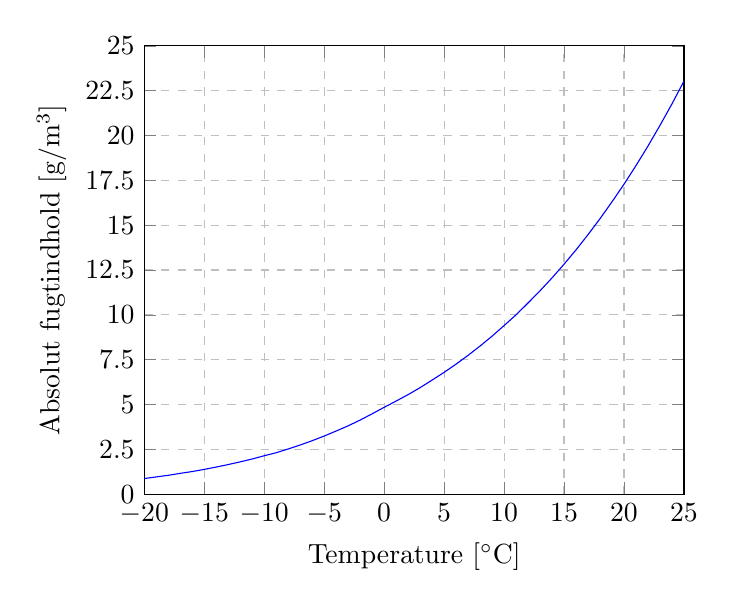
\begin{tikzpicture}
\begin{axis}[
    %title={Luft mættet med vanddamp},
    xlabel={Temperature [$^{\circ}$C]},
    ylabel={Absolut fugtindhold [g/m$^3$]},
    xmin=-20, xmax=25,
    ymin=0, ymax=25,
    xtick={-20, -15, -10, -5, 0, 5, 10, 15, 20, 25},
    ytick={0.0, 2.5, 5.0, 7.5, 10.0, 12.5, 15.0, 17.5, 20.0, 22.5, 25.0},
    %legend pos=north west,
    ymajorgrids=true,
    xmajorgrids=true,
    grid style=dashed,
]
\addplot[
    color=blue,
    mark=dot,
    ]
    coordinates {
        (-20,0.87)
        (-19,0.96)
        (-18,1.05)
        (-17,1.16)
        (-16,1.26)
        (-15,1.38)
        (-14,1.51)
        (-13,1.65)
        (-12,1.80)
        (-11,1.96)
        (-10,2.14)
        (-9,2.31)
        (-8,2.52)
        (-7,2.74)
        (-6,2.98)
        (-5,3.24)
        (-4,3.52)
        (-3,3.81)
        (-2,4.13)
        (-1,4.48)
        (0,4.84)
        (1,5.19)
        (2,5.55)
        (3,5.94)
        (4,6.36)
        (5,6.79)
        (6,7.25)
        (7,7.74)
        (8,8.26)
        (9,8.81)
        (10,9.40)
        (11,10.00)
        (12,10.66)
        (13,11.34)
        (14,12.06)
        (15,12.82)
        (16,13.62)
        (17,14.47)
        (18,15.36)
        (19,16.30)
        (20,17.28)
        (21,18.32)
        (22,19.41)
        (23,20.56)
        (24,21.76)
        (25,23.03)        
    };
    %\legend{g/m$^3$}
\end{axis}
\end{tikzpicture}
\end{center}
\caption{Luft mættet med vanddamp}\label{fig:luft_vanddamp}
\end{figure}
Der bruges en IHC fugt/temperatur sensor, som melder tilbage med en temperature, relativ fugtighed, dugpunkt og et alarm signal.

\subsubsection{Beregning af pumpetiden}\label{subsubsec:beregning_af_pumpetiden}
For at vide hvor langtid pumpen skal køre for, at nå en givet relative fugtighed, 
har jeg lavet en samme regning af hvor mange liter i time og omregning af relative fugtigheden.
Hvis vi tager en avariepumpe som kan lever mellem 170 l/timen - 300 l/timen og omregner det til m$^3$/minut,
så kan det bruges sammen med beregningen af fugtigheden.
Først omregner det timen til minutter
\begin{align}
    \frac{170 \text{ l/t}}{60} &= 2,833 \text{ l/minut} \\
    \frac{300 \text{ l/t}}{60} &= 5 \text{ l/minut}
\end{align}
Herefter omregnes volumnestrømmen fra liter til m$^3$,
\begin{align}
    q_{v_1} &=\frac{2,833 \text{ l/minut}}{1000} = 0,002833 \text{ m$^3$/minut} \\
    q_{v_2} &= \frac{5 \text{ l/minut}}{1000} = 0,005 \text{ m$^3$/minut}
\end{align}
%Da luften kan optage forskellige mængder af vand i forhold til temperature, som en ikke linær funktion.
%For at gøre det nemmere for os selv, så er det valgt at kigge på temperature intervalget 20$^\circ$C til 25$^\circ$C.
%For de værdier, tages der et gennemsnit som der bruges til beregningen
%\begin{align}
%    \frac{17,28 + 18,32 + 19,41 + 20,56 + 21,76 + 23,03}{5} &= 20,06 \text{ g/m$^3$}
%\end{align}
%Det giver selvfølgelig en fejl, men der kun ønskes at have en pumpetid som er i nærheden og da aktiv måles den relative fugtighed. 
%Det betyder under, at vand mængden som bliver optaget af luft kan beregnes.
%\begin{align}
%    &(170 \text{ l/t})\text{ } 0,002833 \text{ m$^3$/min} \cdot 20,06 \text{ g/m$^3$} = 0,05682998 \text{ g/minut} \\
%    &(300 \text{ l/t})\text{ } 0,005 \text{ m$^3$/min} \cdot 20,06 \text{ g/m$^3$} = 0,1003 \text{ g/minut}
%\end{align}
For at kunne beregne den hvor meget vand som skal optages i luften i det give drivhus, så skal volumne kendes. 
Det tal vi får ud af fugtighedsensoren, er relative fugtigthed som er angive i procent. 
Så kan vi skrive
\begin{align}
    t_{on} &= \Delta\%RF\cdot\frac{ V_{\text{drivhus}} }{ q_{v}  } [min]
\end{align}
Det drivhus som kunden har en volumen på 22,75 m$^3$, så giver det
\begin{align}
    t_{on_{1}} & = \Delta\%RF\cdot\frac{ 22,75 }{0,002822} = \Delta\%RF\cdot8061,66 \\
    t_{on_{2}} & = \Delta\%RF\cdot\frac{ 22,75 }{0,005} = \Delta\%RF\cdot4550 
\end{align}
Som det kan ses ud af $t_{on_{1}}$ og $t_{on_{2}}$ så er pumpen i underkanten til, at få fugtighed op i hele drivhuset.
Selv hvis der er en $\Delta\%RF$ på 1\%, så giver det henholdsvis
\begin{align}
    t_{on_{1}} &= \frac{1}{100} \cdot 8061,66 = 80,6166 min \\
    t_{on_{2}} &= \frac{1}{100} \cdot 4550 = 45 min \ 30 sek
\end{align}
og $\Delta\%RF$ kan omskrives til 
\begin{align}
    \Delta\%RF = \frac{ RF_{\text{sætpunkt}} - RF_{\text{målt}} }{ 100 }
\end{align}
Hvis den valgte pumpe stadig ønskes at bruges, så kan man sætte et plastik gardin op foran planterne.
Derved bliv volumen som skal have en høj fugtighed mindre. Hvis volumen halvers, så fåes
\begin{align}
    t_{on_{1}} & = \Delta\%RF\cdot\frac{ 11,375 }{0,002822} = \Delta\%RF\cdot4030,83 \\
    t_{on_{2}} & = \Delta\%RF\cdot\frac{ 11,375 }{0,005} = \Delta\%RF\cdot2275 
\end{align}
Og igen bruger $\Delta\%RF$ på 1\%, så giver det henholdsvis
\begin{align}
    t_{on_{1}} & = \frac{1}{100}\cdot\frac{ 11,375 }{0,002822} = 40 \ min \ 19 \ sek\\
    t_{on_{2}} & = \frac{1}{100}\cdot\frac{ 11,375 }{0,005} = 22 \ min \ 45 \ sek
\end{align}

\subsubsection{Styring}
Til drivhus styring er der valgt, at bruge en Siemens LOGO! 12/24RCE. 
Den er valgt ud fra at den har indbygget 0 - 10 V input, 
som gør det muligt at tilslutte et potentiometer med en flyder på, 
så vandniveauet i regnvandsopsamleren kan måles.

Denne LOGO! enhed har også relæ udgange, 
hvilket gør det muligt at styre flere forskellige spænding niveauer.
Så er det også muligt, at udvide med forskellige 24 V moduler, hvilket ikke er mulig i 230 V versionen.

\subsubsection{Analog indgange}
på side 41 i \cite{logo_sm} og side 42 i \cite{logo_sm} står der omkring modstande til spændingsdeling i LOGO!

        \subsection{Intelligent bygningsinstallation}

\subsubsection{Scenarie i IHC installationen} \label{subsub:ihc_scener}
%\todo{Beskrivelse af de forskellige scenarier}

\paragraph{Velkomst}
Ved et enkelt tryk på kontakten i bryggers, ville lyset tænde ud i bryggers.\\
Ved et langt tryk på samme kontakt, ville lyset tænde i bryggers, 
samt ganglyset og lyset over køkkenbordet.\\
Efter 2 minutter, slukkes lyset i bryggeres og efter yderlig et minut slukkes lyset i gangen.

\paragraph{På vej ud af huset, i bryggers}
Ved et kort tryk slukkes alt lyset i huset undtagen værelserne. 
Lyset i bryggers slukkes efter 2 minutter. \\
Ved et langt tryk slukkes alt lyset i huset samt værelserne. 
Lyset i bryggeres slukkes efter 2 minutter, 
ventilationsanlægget startes på høj udsugning efter 10 minutter og køre efter tidsstyringen. 

\paragraph{Sluk alt lys i huset}
Dette er et scenarie, som ikke er koblet til en kontakt men i stedet bruges af andre scenarie til, 
at slukke for alt i huset med undtagelse af værelserne og soveværelset.

\paragraph{Godnat scenarie i soveværelse}
Ved et kort tryk på kontakten ved sengen, 
så slukkes lyset soveværelset og i resten af huset med undtagelse af værelserne.\\
Ved et langt tryk på kontakten ved sengen, 
så slukkes alt lyset i huset også i alle værelserne.

\paragraph{Godnat scenarie i resterende værelse}
Ved et kort tryk på kontakten ved sengen, 
så slukkes lyset soveværelset og i resten af huset med undtagelse af andre værelser og soveværelset. \\
Ved et langt tryk på kontakten ved sengen, 
så slukkes alt lyset i huset også i alle værelserne samt soveværelset.

\paragraph{Tidsstyring af ventilationsanlægget}
I hverdage ville anlægget blive startet på høj udsugning kl 10.00 hvis ud af huset ikke er blevet aktiveret inden. 
Ventilationsanlægget ville køre i en 1 time hvor efter den ville køre ned på lav hastighed. \\
Her efter ville anlægget startes på høj udsugning kl 13.00 (efter frokost) køre en halv time hvorefter den igen går ned på lav hastighed.
Igen kl 19 ville anlægget starte på høj udsugning (efter aftensmaden) køre en halv time på høj og gå ned på lav hastighed.

\paragraph{Overstyring af ventilationsanlægget}
Hvis luftfugtigheden på badværelset bliver over 30\%, så startes ventilationsanlægget på høj udsugning til luftfugtigheden er faldet til 20 \% igen. \\
Ved at trykke på den nederest kontakt til højre i køkkenet, ville ventilationsanlægget start på høj udsugning. Ved at trykke på samme kontakt ville anlægget stoppe. \\
Ved at trykke på den nederest kontakt til højre i bryggers, ville ventilationsanlægget start på høj udsugning. Ved at trykke på samme kontakt ville anlægget stoppe.

%\subsubsection{Styring af udsugning i drivhuset} \label{subsub:ihc_drivhus}
%\todo{Beskrive hvordan styring af fugten i drivhuset}
%\todo{Hvis fugtigtheden falder til under 60 \%, starter styringen. Hvis den er over 80 \% stopper styringen}
%Da IKEA's Trådfri app kun kan lave den mest basale styringen og ikke det som kunden til efterspørger. Så er vi ``tvunget`` til at kigge på nogle lidt andre løsningen end de meste standarde løsningen.

%\subsubsection{Home-Assistant}
%Home-Assistant (\cite{HAW:2018:Online}) gør det muligt, at samle flere typer af smart bygningsinstallationer under en styring.
%Det er muligt, at bruge IKEA Trådfri sammen med en IHC styring (det kræver dog, at IHC er på netværket). Den understøtter flere forskellige systemer og bliver hele tide udvidet med nye systemer.
%Varmestyringen kan også integeres i denne løsningen, samt egne udviklet enheder kan også blive integret sammen med den. 
%Dette system kan installeres på en minicomputer så for eksemple en Raspberry Pi 3. Når hele systemet er sat op med de enheder som er i installationen, så kan det tilgåes fra en hjemmeside som i modsætning af IHC controlleren ikke er lavet af JAVA.
%Her er det valgt at bruge en Raspberry Pi 3 model b+, og det er den billed-fil af hass.io som også er blevet hentet ned.
        \subsection{Ventilation} \label{sub:ventilation}
Der tages udgangspunkt i BR18 [\cite{BR18:Online}] kravene.
Under \S443 står kravene beskrevet at der skal være en udelufttilførsel på mindst 0,3 l/s pr. m$^2$.
I \S443 stk. 3 står der at udsugningen i køkkener skal forøges til mindst 20 l/s og \S443 stk. 4 beskriver udsugningen fra bade- og wc-rum skal kunne forøges til mindst 15 l/s.
Desuden beskreves der også at wc-rum uden bad og bryggers skal der kunne udsuges mindst 10 l/s. 
I forhold til BR15 så der ikke nogle ændring i kravene som har betydning for beregningen.
Dog beskriver BR18, i \S444 at kælder i enfamileshus skal der udsuges mindst 10 l/s.

\subsubsection{Bestemmelse af minimumskravet til anlægget} \label{subsub:minimumkrav_ventilation}
Da kravene for lufttilførelsen kun gælder for de opvarmet beboelse kvm,
det betyder at ydre vægge ikke behøves at være med i udregningen.
I BR18 [\cite{BR18:Online}], 
så skal udelufttilførsel minimum være med 0,3 l/s pr. m$^2$ opvarmet etageareal.
For at kunne lave beregningen, så skal det udregnes til en volumenstrømmen som er i m$^3$/t. 
Dette gøres med at gange 3,6 $\frac{ \text{m}^3 \text{/ l} }{\text{ t / s} }$ for at omregne fra sekunder til timer og liter til kubicmeter.
i tabel \ref{table:samregn_vent_ind} på side \pageref{table:samregn_vent_ind} har jeg regnet ud fra rummenes kvm.

\begin{table}[!h]
     \begin{center}
        \begin{tabular}{|l|r|r|r|}
            \hline
            Rum & kvm & Udelufttilførsel i l/s & Udelufttilførsel i m$^3$/t \\
            \hline
            Soveværelse       & 12,6 m$^2$ & 3,78 l/s & 13,61 m$^3$/t\\
            Stue / Alrum / Køkken & 39,7 m$^2$ & 11,91 l/s & 42,88 m$^3$/t\\
            Entré / Bryggers  & 9,6 m$^2$ & 2,88 l/s & 10,37 m$^3$/t\\
            Gang              & 2,3 m$^2$ & 0,69 l/s & 2,48 m$^3$/t\\
            Værelse 1         & 11,9 m$^2$ & 3,57 l/s & 12,85 m$^3$/t\\
            Værelse 2         & 12,0 m$^2$ & 3,60 l/s & 12,96 m$^3$/t\\
            Bad 1             & 4,3 m$^2$ & 1,29 l/s & 4,64 m$^3$/t\\
            Bad 2             & 7,5 m$^2$ & 2,29 l/s & 8,24 m$^3$/t\\
            \hline
            \hline
            Samlet & \underline{99,9 m$^2$} & \underline{30,01 l/s} & \underline{108,03 m$^3$/t} \\
            \hline
        \end{tabular}
    \end{center}
    \caption{Udregning af Udelufttilførelsens minimumskrav}
    \label{table:samregn_vent_ind}
\end{table}

Så vores krav til udelufttilførsel er at anlægget skal kunne minimum lave et luftskifte på 30,01 l/s.
I BR18 [\cite{BR18:Online}] beskreves der også hvor meget luft som skal udsuges i udvalgte rum, 
de tal skal ligges sammen og ud fra det kan laves en sammenregning til minimumskravet. De udregning findes i tabel \ref{table:samregn_vent_ud} på side \pageref{table:samregn_vent_ud}.
\begin{table}[!h]
    \begin{center}
       \begin{tabular}{|l|r|r|}
           \hline
           Rum & Udsugning i l/s & Udsugning i m$^3$/t \\
           \hline
           Stue / Alrum / Køkken & 20 l/s & 72 m$^3$/t\\
           Entré / Bryggers  & 15 l/s & 54 m$^3$/t\\
           Bad 1             & 15 l/s & 54 m$^3$/t\\
           Bad 2             & 15 l/s & 54 m$^3$/t\\
           \hline
           \hline
           Samlet & \underline{65 l/s} & \underline{234 m$^3$/t} \\
           \hline
       \end{tabular}
   \end{center}
   \caption{Udregning af udsugnings minimumskrav}
   \label{table:samregn_vent_ud}
\end{table}
Her kan det ses, at minimumskrav til udsugning er højere end til udelufttilførselen. 
Da der ønskes, at der er en ligevægt i ens ventilationssystem så beregnes rør diameteren udfra minimum volumenstrømmen i udsugningen.
\begin{equation}\label{eqn:udregning_rd}
d_{n} = \sqrt{ \frac{q_{v} \cdot 4}{V\cdot\pi\cdot3600}}
\end{equation}
Ligning (\ref{eqn:udregning_rd}) på side \pageref{eqn:udregning_rd} bruges til, udregne diameteren i meter, $V$ er lufthastigheden i $m/s$ og $q_v$ er volumenstrømmen i $m^{3}/t$.
Typisk er lufthastigheden mellem 4 - 10 m/s. 
\begin{align} \label{eqn:udregning_min_rd} 
    d_{n}       &= \sqrt{ \frac{q_{v} \cdot 4}{V\cdot\pi\cdot3600}} = \sqrt{ \frac{234 \cdot 4}{4\cdot\pi\cdot3600}} = 0,1438 m = 143,8 mm
\end{align}
Beregningen af rørdiameteren i ligning (\ref{eqn:udregning_min_rd}) på side \pageref{eqn:udregning_min_rd} er fundet til 143,8 mm, 
ikke findes i lindab's sortiment så vælges rørdiameteren til 160mm.

\subsubsection{Tryktab i udsugning} \label{subsub:tryktab_udsugning}
Der er en oversigts tegning over ventilationssystem på side \pageref{fig:tegning_ventr}. 
Længderne er skrevet på tabel \ref{table:oversigt_l_udsugning} på side \pageref{table:oversigt_l_udsugning}, 
der er også valgt at inkludere hvilket volumenstrømmen som skal være i de enkelte rør. 
\begin{align} \label{eqn:volumenstroem_sammenregning} 
    q_{v}(E) &= q_{v}(F) + q_{v}(H) = 54 + 54 = 108 \text{ m}^3\text{/t}
\end{align}
Alle volumenstrømmene skal omregnes til lufthastighed, 
for at kunne finde frem til tryk tabet i rørene, 
det gøres i ligningen \ref{eqn:omregning_vs_til_lh}.
\begin{align} \label{eqn:omregning_vs_til_lh}
    d_{n} &= \sqrt{ \frac{ q_v \cdot 4 }{ V\cdot \pi \cdot 3600 } }  \nonumber \\
          &\Downarrow  \nonumber \\
    d_{n}^{2} &= \frac{ q_v \cdot 4 }{ V\cdot \pi \cdot 3600 } \nonumber \\
          &\Downarrow \nonumber \\
    V     &= \frac{ q_v \cdot 4 }{ d_{n}^{2} \cdot \pi \cdot 3600 } 
\end{align}
Ved at bruge formulen i \ref{eqn:omregning_vs_til_lh}, 
giver den lufthastighed som bruges til, 
at finde tryktabet per meter i databladet for røret.
\begin{table}[h!]
    \begin{center}
       \begin{tabular}{|l|r|r|r|r|r|}
           \hline
           Længde & meter & q$_{v}$ & V & P$_{a}$ / m & Tryktab\\
           \hline
           A & 1,38 m & 270 m$^3$/t & 3,73 m/s & 1,2 P$_{a}$/m & 1,656 Pa\\
           B & 0,27 m & 162 m$^3$/t & 2,24 m/s & 0,5 P$_{a}$/m & 0,135 Pa\\
           C & 0,75 m & 72  m$^3$/t & 0,99 m/s & 0,1 P$_{a}$/m & 0,075 Pa\\
           D & 4,43 m & 54  m$^3$/t & 0,75 m/s & 0,1 P$_{a}$/m & 0,443 Pa\\
           E & 0,46 m & 108 m$^3$/t & 1,49 m/s & 0,2 P$_{a}$/m  & 0,092 Pa\\
           F & 0,94 m & 54 m$^3$/t & 0,75 m/s & 0,1 P$_{a}$/m & 0,094 Pa\\
           G & 2,79 m & 54 m$^3$/t & 0,75 m/s & 0,1 P$_{a}$/m & 0,279 Pa\\
           H & 0,45 m & 54 m$^3$/t & 0,75 m/s& 0,1 P$_{a}$/m & 0,045 Pa\\
           \hline
       \end{tabular}
   \end{center}
   \caption{Oversigt over længderne brugt i udsugningen}
   \label{table:oversigt_l_udsugning}
\end{table}
I tabel \ref{table:oversigt_l_udsugning}, er lufthastigheden som skal bruges til at finde tryktabet i T-rørene.
Dette gøres ved, at aflæse graferne i databladet for T-stykkerne.
\begin{table}[h!]
    \begin{center}
       \begin{tabular}{|l|r|r|r|}
           \hline
           T-rør & V$_{1}$ & V$_{2}$ & Tryktab \\
           \hline
           T$_{\text{B->A}}$ & 2,24 m/s & 3,73 m/s & 4,8 Pa \\ 
           T$_{\text{C->A}}$ & 0,99 m/s & 3,73 m/s & 2,8 Pa \\
           T$_{\text{E->B}}$ & 1,49 m/s & 2,24 m/s & 0,6 Pa \\
           T$_{\text{D->B}}$ & 0,75 m/s & 2,24 m/s & 1,5 Pa \\
           T$_{\text{F->E}}$ & 0,75 m/s & 1,49 m/s & 0,8 Pa \\
           T$_{\text{G->E}}$ & 0,75 m/s & 1,49 m/s & 1,0 Pa \\
           \hline
       \end{tabular}
   \end{center}
   \caption{Oversigt tryktabet i T-rør}
   \label{table:oversigt_tryktab_t-roer}
\end{table}
Nu kan tryktabet findes på det stykke som er længes væk fra ventilationsanlægget, 
som er rum bad 2.
\begin{table}[h!]
    \begin{center}
       \begin{tabular}{lcr}
           \hline
           \hline
           \textbf{Bad 2} &  & \\
           \hline
           \hline
           Ventil (-5mm åbning) & : & 21,000 Pa \\
           90$^\circ$ BU    & : & 0,500 Pa \\
           Rør$_{\text{H}}$ & : & 0,045 Pa \\
           90$^\circ$ BU    & : & 0,500 Pa \\
           Rør$_{\text{G}}$ & : & 0,279 Pa \\
           T-Stykke$_{\text{G->E}}$  & : & 1,000 Pa\\
           Rør$_{\text{E}}$ & : & 0,092 Pa \\
           T-Stykke$_{\text{E->B}}$  & : & 0,600 Pa\\
           Rør$_{\text{B}}$ & : & 0,135 Pa \\
           T-Stykke$_{\text{B->A}}$  & : & 4,800 Pa\\
           Rør$_{\text{A}}$ & : & 1,656 Pa \\
           \hline
           Samlet tryktab    & : & \underline{\underline{ 30,607 Pa}} 
       \end{tabular}
   \end{center}
   %\caption{Oversigt tryktabet i T-rør}
   %\label{table:oversigt_tryktab_t-roer}
\end{table}

\subsubsection{Tryktab i indblæsning} \label{subsub:tryktab_indblaesning}
I tabel \ref{table:oversigt_l_indblaesning}, beskriver længderne brugt til indblæsningen. 
Lufthastighed, Tryktab per meter beskrevet i tabellen er fundet ved hjælp af lindab's App `Vent Tools',
og tryktabet er herefter udregnet fra de tal.
\begin{table}[h!]
    \begin{center}
       \begin{tabular}{|l|r|r|r|r|r|}
           \hline
           Længde & meter & q$_{v}$ & V & P$_{a}$ / m & Tryktab\\
           \hline
            P & 3,94 m & 13,61 m$^3$/t & 0,19 m/s & 0,0 P$_{a}$/m & 0 Pa\\
            O & 0,74 m & 13,61 m$^3$/t & 0,19 m/s & 0,0 P$_{a}$/m & 0 Pa\\
            N & 4,71 m & 56,49 m$^3$/t & 0,78 m/s & 0,1 P$_{a}$/m & 0,471 Pa\\
            M & 4,24 m & 12,96 m$^3$/t & 0,18 m/s & 0,0 P$_{a}$/m & 0 Pa\\
            K & 3,50 m & 25,81 m$^3$/t & 0,36 m/s & 0,0 P$_{a}$/m & 0 Pa\\
            J & 1,78 m & 82,30 m$^3$/t & 1,14 m/s & 0,1 P$_{a}$/m & 0,178 Pa\\
            I & 0,74 m & 82,30 m$^3$/t & 1,14 m/s & 0,1 P$_{a}$/m & 0,074 Pa\\
           \hline
       \end{tabular}
   \end{center}
   \caption{Oversigt over længderne brugt i indblæsning}
   \label{table:oversigt_l_indblaesning}
\end{table}
Tryktabet i T-stykkerne er beskrevet i tabel \ref{table:oversigt_tryktab_t-roer_ind}. 
Lufthastighed for Stue/Alrum/Køkken og Værelse 1 er beregnet ud fra \ref{eqn:omregning_vs_til_lh} på side \pageref{eqn:omregning_vs_til_lh}.
Stue's udregning kan se i udregning \ref{eqn:udregning_af_vs_stue}.
\begin{align} \label{eqn:udregning_af_vs_stue}
    V     &= \frac{ q_v \cdot 4 }{ d_{n}^{2} \cdot \pi \cdot 3600 } \nonumber \\
    V     &= \frac{ 42,88 \cdot 4 }{ (160/1000)^{2} \cdot \pi \cdot 3600 } \nonumber \\
    V     &= \frac{ 171,53 }{ 92,16 \cdot \pi } \nonumber \\
    V     &= 0,592 \text{ m/s}
\end{align}
Når der aflæses i databladet for T-stykkerne, så er det udenfor skalaen.
Det kommer af, at rørdiameteren er sat efter udsugning det sætter lufthastigheden ned og derfor kan tabet sættes til 0 Pa.
Det betyder, at indblæsningen ikke ville have noget tab af betydning i T-stykkerne.
\begin{table}[h!]
    \begin{center}
       \begin{tabular}{|l|r|r|r|}
           \hline
           T-rør & V$_{1}$ & V$_{2}$ & Tryktab \\
           \hline
           T$_{\text{J->N}}$ & 1,14 m/s & 0,78 m/s & 0 Pa \\ 
           T$_{\text{J->K}}$ & 1,14 m/s & 0,36 m/s & 0 Pa \\ 
           T$_{\text{N->O}}$ & 0,78 m/s & 0,19 m/s & 0 Pa \\ 
           T$_{\text{N->Stue}}$ & 0,78 m/s & 0,59 m/s & 0 Pa \\ 
           T$_{\text{K->M}}$ & 0,36 m/s & 0,18 m/s & 0 Pa \\ 
           T$_{\text{K->Værelse 1}}$ & 0,36 m/s & 0,71 m/s & 0 Pa \\ 
           \hline
       \end{tabular}
   \end{center}
   \caption{Oversigt tryktabet i T-rør for indblæsning}
   \label{table:oversigt_tryktab_t-roer_ind}
\end{table}
Nu kan tabet findes på den længeste strækning. Som er på indblæsning er soveværelset.
\begin{table}[h!]
    \begin{center}
       \begin{tabular}{lcr}
           \hline
           \hline
           \textbf{Soveværelse} &  & \\
           \hline
           \hline
           Ventil (6mm åbning) & : & 15,000 Pa \\
           90$^\circ$ BU    & : & 0 Pa \\
           Rør$_{\text{P}}$ & : & 0 Pa \\
           90$^\circ$ BU    & : & 0 Pa \\
           Rør$_{\text{O}}$ & : & 0 Pa \\
           T-Stykke$_{\text{N->O}}$  & : & 0 Pa\\
           Rør$_{\text{N}}$ & : & 0,471 Pa \\
           T-Stykke$_{\text{J->N}}$  & : & 0 Pa\\
           Rør$_{\text{J}}$ & : & 0,178 Pa \\
           90$^\circ$ BU    & : & 3,800 Pa \\
           Rør$_{\text{I}}$ & : & 0,074 Pa \\
           \hline
           Samlet tryktab & : & \underline{\underline{ 19,523 Pa}} 
       \end{tabular}
   \end{center}
   %\caption{Oversigt tryktabet i T-rør}
   %\label{table:oversigt_tryktab_t-roer}
\end{table}

\subsubsection{Valg af ventilationsaggregater}
\todo{Valgt Beskrive hvordan der skal vælgees}

%    \section{Perspetivering}
  
%    \section{Konklusion}
    \section{Konklusion}
Drivhus styringen som er blevet implementeret viser, 
at der kan findes en løsning med komponenter som ikke er beregnet til at kommuniker sammen.
I dette tilfælde IHC fugt- og temperatur sensoren brugt inde i drivhus hvorefter dens værdi,
bliver kommuniker videre til styringen. En bedre løsning ville være, at bruge en anden sensor
som er designet til det høje luftigheds miljø. 
\\ \\
Grunden til, at vælge en intelligent bygningsinstallation er at øge ens comfort. 
At få automatiseret blandt andet lyset efter funktionen af rummet, kører forceret drift på ventilationsanlægget
når man ikke er hjemme. 
Eller bruge en fugt sensor i på badværelset, hvis den relative fugt niveau kommer over de 30\% at ventilationsanlægget køre op i hastighed.
Der bruges en IHC controller til lysstyringen, og der ønskes at ventilationsanlægget kan styres igennem IHC.

Det betyder, at i valgt af ventilationsanlægget skal der tages højde for at dens styring kan overstyres af en ekstern enhed.
Ventilationsproducent Nilan har lavet en styring (CTS 602) som har en funktionsblok i IHC, 
hvilket gøre det mere simple at få kommunikationen til at virke mellem de to styringer.
I tilbuddet er der valgt et Nilan Comfort 600 med en CTS 602 styring, så integrationen i IHC styring er dokumenteret fra producentes side.


%.tex}

    \appendix
    \section{Projektbeskrivelse}
\textbf{Dato:} \today \\
\textbf{Navn:} Michael Torp Kaalund\\
\textbf{Valg af moduler i uddannelsen:}
\begin{itemize}
    \item Modul 1.3 Automatiske anlæg i bygninger
    \item Modul 1.4 Intelligente bygningsinstallationer (centrale) og design af enkle brugerflader
    \item Modul 1.6 Design og styring af lys
    \item Modul 2.2 Styring og regulering af automatiske anlæg
\end{itemize}
\textbf{Moduler, der indgår i svendeprøven:}
\begin{itemize}
    \item Modul 1.3 Automatiske anlæg i bygninger
    \item Modul 1.4 Intelligente bygningsinstallationer (centrale) og design af enkle brugerflader
    \item Modul 2.2 Styring og regulering af automatiske anlæg
\end{itemize}
\textbf{Klasse:} elsp4d18

\begin{enumerate}
    \item \textbf{Angiv hvem der har ansvar for hvilke områder af projektet, hvis der arbejdes i en
    gruppe:}\\ Da jeg har valgt, at arbejde alene. Så det fulde ansvar er hos mig.
    \item \textbf{Problemstilling og formål med projektet:} \\ 
    Kunden ønsker at få et automatiseret drivhus styring. Som
    automatisk fylder vand i planteboksene fra hans regnvandsopsamling.
    Styringen skal kunne holde et konstant niveau i plantekasserne. \\
    Kunden får lavet en lysinstallation med IHC. 
    %Kunden har et ønske om, at få en lysstyring som både kan styre den IHC og
    %IKEA Trådfri / Philips HUE. 
    \\
    Kunden ønsker også, at ventilationsanlægget, skal kunne komme ind over styringen.
    Hvordan kan det være muligt, at lave kommunkation som kan over flere flader?
    % (f.eks IHC, IKEA Trådfri, ventilationsanlægget osv.)\newcounter{enumi_saved}

    \item \textbf{Indhold af projektet, herunder mulige tekniske løsningsmodeller} \\ 
    Med den tid som er tilrådighed ville det blive presset hvis der skulle laves og dokumenteres installationen og programmingerne af et helt hus, samt design af drivhus styringen. 
    Drivhus styring ville der blive lagt vægt på samt hvordan en intelligent bygningsinstallation kunne programmeres op.
    Det innovative del af projektet er automatisering af drivhuset i en privat bolig. Selv om der har fået et fremryk de seneste par år, med en smart lysstyring i bolig, så er det langt fra alle løsninger som er optimale i forhold til hvordan brugeren udnytter dette. 
    \\
    Vandstyringen til drivhusstyringen
    \begin{itemize}
        \item Siemens LOGO! 12/24RCE
        \item Siemens LOGO! Power 24V 2,5A
        \item Akvarie Pumpe
        \item 2 stk Vandniveau måler med 0 - 10V udgang, eller et potentiometer ( $5k\Omega$) og en serie modstand ($6,6k\Omega$) \footnote{Side 42 \cite{logo_sm} }
        \item Tavle med din skinne eller montage boks med din skinne.
        \item $3g1,5mm^2$ tilledning
        \item 3pol stikprop
        \item C6A automatsikring eller en B10A automatsikring.
        \item Sløjfeledning $1mm^2 - 2,5mm^2$
    \end{itemize}
    Eventuelle udstyr til lysstyring
    \begin{itemize}
        \item IHC controller
        \item IHC strømforsyning
        \item IHC 230V output relæ
%        \item IKEA Trådfri pære 3 stk
%        \item IKEA Trådfri tryk
%        \item IKEA Trådfri gateway
        \item WiFi Router inkl. switch
%        \item Raspberry PI 3 model B+
%        \item 5V 2,5A strømforsyning (usb lader)
%        \item Nilan Comform 300 ventilationsanlægget med CTS602
%        \item Nilan Connect 
        \item IHC input 24/3
        \item IHC output 24
        \item IHC Fugt sensor
    \end{itemize}

    \item \textbf{Beskrivelse af opgaver eller installationer, der kan demonstrere dine tekniske,
    håndværksmæssige og innovative færdigheder} \\ 
    Der ville opbygges en test opstilling af drivhusstyringen. Der ville blive lavet en tegning og en beregning af ventilationsanlægget, samt der ville beskrivelse hvordan styringen kan automatiseret. Der ville beskrivelses hvordan der ville kunne være en central styringen til lysinstallation.
 
    \item \textbf{Forslag til dokumentation for de valgte løsninger.}
    \begin{itemize}
        \item Brugervejledning.
        \item Tekniske tegninger.
        \item Relevante beregninger.
        \item Beskrivelse af love og regler som er gældene.
    \end{itemize}
    \item \textbf{Tidsstyring af projektet:}
    \begin{itemize}
        \item Den budgeteret tidsplan, ville blive opsat i Microsoft Excel eller i et lignene program.
        \item Der ville også blive lavet en realiseret tidsplan i samme format.
        \item Der ville blive lavet en status ved afslutning af arbejdsdagen.
    \end{itemize}
   
\end{enumerate}   
    \section{Tidsplan forventet} \label{sec:tidsplan_forventet}
    \includegraphics[scale=0.72,angle=270,origin=c]{appendix/tidsplan_forventet.pdf}
    %\newpage
    \section{Tidsplan realiseret} \label{sec:tidsplan_realiseret}
    \includegraphics[scale=0.72,angle=270,origin=c]{appendix/tidsplan_realiseret.pdf}
    %\section{Tidsplan forventet} \label{sec:tidsplan_forventet}
\includegraphics[scale=0.75,angle=270,origin=c]{appendix/tidsplan_forventet.pdf}
%\newpage
\section{Tidsplan realiseret} \label{sec:tidsplan_realiseret}
\includegraphics[scale=0.75,angle=270,origin=c]{appendix/tidsplan_realiseret.pdf}
    \section{Materialeliste} 
    \includegraphics[scale=0.72,angle=270,origin=c]{appendix/materialeliste/bom_1.pdf}
    \newpage
    \includegraphics[scale=0.72,angle=270,origin=c]{appendix/materialeliste/bom_2.pdf}
    %\documentclass[12pt,a4paper,twoside,landscape]{article}
    \special{papersize=210mm,297mm}
    
    \usepackage[a4paper,includeheadfoot,margin=2.54cm]{geometry}
    \usepackage{pdflscape}
    \usepackage{hyperref}
    \usepackage{natbib}
    \bibliographystyle{plainnat}

    \usepackage[utf8]{inputenc}
    \usepackage{graphicx}
    \usepackage[danish]{babel}

    \usepackage[familydefault,regular]{Chivo}
    \usepackage[T1]{fontenc}

    \usepackage{lastpage}
    \usepackage{fancyhdr}
    \usepackage{xcolor}
    \usepackage{mathtools}
    \usepackage{amsmath}
    \usepackage{gensymb}
    %Plotning af 
    \usepackage{pgfplots}
    \usepackage{pdfpages}
    %\pgfplotset{width=10cm,compat=1.9}
    \usepackage{multirow}     
    %\usepackage{tabularx}
    \usepackage{booktabs}% http://ctan.org/pkg/booktabs
    \newcommand{\tabitem}{~~\llap{\textbullet}~~}

    \newcommand{\todo}[1]{\textcolor{red}{TODO: #1}\PackageWarning{TODO:}{#1!}}
                 
    \pagestyle{fancy} 
    \fancyhf{}
    %\fancyhead[LE,RO]{Et kig på IBI i privaten}
    %\fancyhead[RE,LO]{\rightmark}
    \fancyfoot[CE,CO]{ }
    \fancyfoot[LE,RO]{ }
    \renewcommand{\headrulewidth}{0pt}
    \renewcommand{\footrulewidth}{0pt}
 
    %% Ny 
    \newcommand{\vdc}{V$_{\text{DC}}$ }
    \newcommand{\vac}{V$_{\text{AC}}$ }

    %\title{Et kig på IBI i privaten}
    
    %\author{Michael Torp Kaalund \thanks{Mange tak til min læreplads Intego A/S}}
    
    \begin{document}


\begin{tabular}[c]{|l|l|l|r|c|r|}
    \hline
    & Butik & Beskrivelse & Pris pr. stk. & Antal & Samlet pris \\
    \hline \hline
    \parbox[t]{2mm}{\multirow{7}{*}{\rotatebox[origin=c]{90}{Drivhus Styring}}}& Plantorama Randers & Eheim CompactOn 300 &  kr. 103,20 & 1 & kr. 103,20 \\
    & Plantorama Randers & SF Akvarieslange Ø9/12 3 meter & kr. 35,96 & 1 & kr. 35,96 \\
    & Lemvigh-Müller & Siemens LOGO! 12/24RCE & kr. 1048,38 & 1 & kr. 1048,38 \\
    & Lemvigh-Müller & Siemens LOGO!Power 24V/2,5A &  kr. 547,03 & 1 & kr. 547,03 \\
    & Lemvigh-Müller & Gennemgangsklemme WDU2,5 Grå & kr. 8,19 & 25 & kr. 204,75 \\
    & Lemvigh-Müller & Gennemgangsklemme WDU2,5 Blå & kr. 8,19 & 5 & kr. 40,95 \\
    & Lemvigh-Müller & Gennemgangsklemme WDU2,5 Gul & kr. 8,54 & 5 & 42,70 \\
    \hline \hline
    \parbox[t]{2mm}{\multirow{7}{*}{\rotatebox[origin=c]{90}{IBI installation}}}& Lemvigh-Müller & IHC strømforsyning 72W/24\vdc & kr. 1425,79 & 1 & kr. 1425,79 \\
    & Lemvigh-Müller & IHC Visual Controller med viewer & kr. 6868,18 & 1 & kr. 6868,18 \\
    & Lemvigh-Müller & IHC Udgangsmodul med 8 udgange relæ & kr. 1188,40 & 1 & kr. 1188,40 \\
    & Lemvigh-Müller & IHC Udgangsmodul 400/8x10 & kr. 1584,49 & 1 & kr. 1584,49 \\
    & Lemvigh-Müller & IHC Control Kabel LINK-10 (5x2x0,6) & kr. 11,09 & 100 & kr. 1109,00 \\
    & Lemvigh-Müller & IHC W Fuga batteritryk 4SL Hvid & kr. 600,35 & & \\
    & Lemvigh-Müller & IHC control fugt- og temperatursensor & kr. 777,57 & & \\

    \hline \hline
    &                 & Samlet pris ekls. moms &  & & kr. 2022,97 \\
    &                 & Moms (25 \% ) & & & kr. 505,74 \\
    &                 & Samlet pris inkl. moms & & & kr. 2528,71 \\
                    \hline

\end{tabular}

%\begin{landscape}
    %\thispagestyle{landscapestyle}
    
    %\subsection{Drivhus styring}

I kundens drivhus skal der dyrkes tomater og agurker som har fordel af en relativ luftfugtighed på 70\% - 80\%.
Da dette drivhus ikke er opvarmet, så bliver tomatplanterne udplantet omkring den 1. maj og agurk planterne i slutningen af maj.
Temperaturen i drivhus bør i dagstimerne være mellem 20$^\circ$C - 30$^\circ$C, og helst ikke meget over, da planterne ikke kan holde til varmen.

\subsubsection{Luftfugtighed}
Luftfugtighed fortæller hvor mange gram vand der er i en m$^3$ luft ved en given temperatur.
Hvis vi kigger på figure \ref{fig:luft_vanddamp}, så kan der ses at mængden af vand som luften kan optage er en konstant, men er afhængelige af temperaturen.
Det kan også ses at det ikke er en linære afhængelig af temperaturen.
Så tit ville man bruge relativ luftfugtighed (angivet som \%RF eller \%RH), som angiver luftfugtighed som en er procentsats. 
Da enheden bliver temperatur uafhængeligt og siger om hvor meget vand der i forhold til luften.

%Tomat i drivhus uden varme er fra omkring 1. maj
%Agurk i drivhus uden varme og som små planter i slutningen af maj til juni.

%Begge planter kan ikke klar temperature over 30 grader celcius.

%Luftfugtighed ønskes til at være omkring.

%Reduktion af Luftfugtighed kan ske via ventilation. \url{http://pure.au.dk/portal/files/42028244/743458.pdf}
%Luftfugtighed agurk: 2 g kg$^{-1}$ 
%Luftfugtighed tomat: 3 g kg$^{-1}$ 
%80 \% RH

%\url{https://www.havenyt.dk/spoergsmaal/drivhuset/12188.html}
%Tomater: 20 grader om dagen
%Agurk: 26 - 28 grader om dagen
%\url{https://voresvilla.dk/haven/drivhus-orangeri/undga-sygdomme-drivhuset/}
%Op til 4 liter vand om dagen.
%\url{http://old.gyproc.dk/files/Gyproc/Library/Handbook/DK/HB9%20-%204.5.2%20-%20Fugt%20i%20luft.pdf}
%\url{http://www.vitavia.dk/filarkiv/pdf/Vitavia_broc_2017_DK_low.pdf}

\begin{figure}[!h]
    \begin{center}
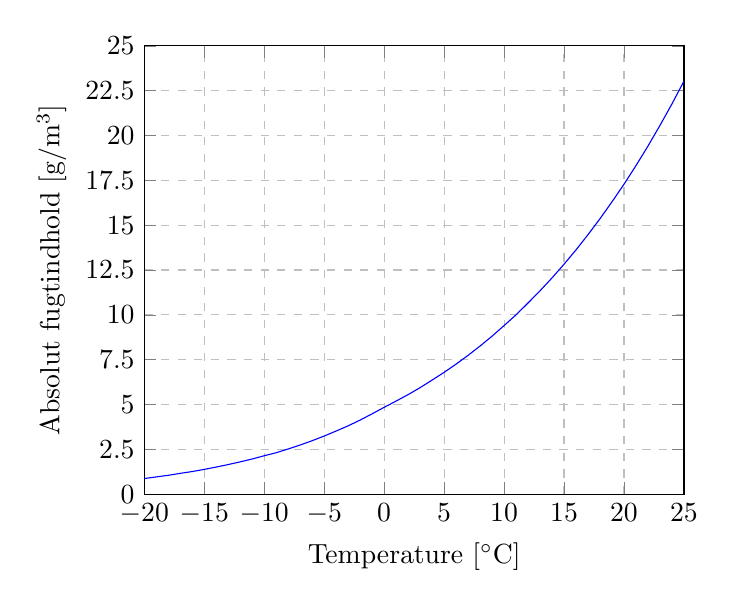
\begin{tikzpicture}
\begin{axis}[
    %title={Luft mættet med vanddamp},
    xlabel={Temperature [$^{\circ}$C]},
    ylabel={Absolut fugtindhold [g/m$^3$]},
    xmin=-20, xmax=25,
    ymin=0, ymax=25,
    xtick={-20, -15, -10, -5, 0, 5, 10, 15, 20, 25},
    ytick={0.0, 2.5, 5.0, 7.5, 10.0, 12.5, 15.0, 17.5, 20.0, 22.5, 25.0},
    %legend pos=north west,
    ymajorgrids=true,
    xmajorgrids=true,
    grid style=dashed,
]
\addplot[
    color=blue,
    mark=dot,
    ]
    coordinates {
        (-20,0.87)
        (-19,0.96)
        (-18,1.05)
        (-17,1.16)
        (-16,1.26)
        (-15,1.38)
        (-14,1.51)
        (-13,1.65)
        (-12,1.80)
        (-11,1.96)
        (-10,2.14)
        (-9,2.31)
        (-8,2.52)
        (-7,2.74)
        (-6,2.98)
        (-5,3.24)
        (-4,3.52)
        (-3,3.81)
        (-2,4.13)
        (-1,4.48)
        (0,4.84)
        (1,5.19)
        (2,5.55)
        (3,5.94)
        (4,6.36)
        (5,6.79)
        (6,7.25)
        (7,7.74)
        (8,8.26)
        (9,8.81)
        (10,9.40)
        (11,10.00)
        (12,10.66)
        (13,11.34)
        (14,12.06)
        (15,12.82)
        (16,13.62)
        (17,14.47)
        (18,15.36)
        (19,16.30)
        (20,17.28)
        (21,18.32)
        (22,19.41)
        (23,20.56)
        (24,21.76)
        (25,23.03)        
    };
    %\legend{g/m$^3$}
\end{axis}
\end{tikzpicture}
\end{center}
\caption{Luft mættet med vanddamp}\label{fig:luft_vanddamp}
\end{figure}
Der bruges en IHC fugt/temperatur sensor, som melder tilbage med en temperature, relativ fugtighed, dugpunkt og et alarm signal.

\subsubsection{Beregning af pumpetiden}\label{subsubsec:beregning_af_pumpetiden}
For at vide hvor langtid pumpen skal køre for, at nå en givet relative fugtighed, 
har jeg lavet en samme regning af hvor mange liter i time og omregning af relative fugtigheden.
Hvis vi tager en avariepumpe som kan lever mellem 170 l/timen - 300 l/timen og omregner det til m$^3$/minut,
så kan det bruges sammen med beregningen af fugtigheden.
Først omregner det timen til minutter
\begin{align}
    \frac{170 \text{ l/t}}{60} &= 2,833 \text{ l/minut} \\
    \frac{300 \text{ l/t}}{60} &= 5 \text{ l/minut}
\end{align}
Herefter omregnes volumnestrømmen fra liter til m$^3$,
\begin{align}
    q_{v_1} &=\frac{2,833 \text{ l/minut}}{1000} = 0,002833 \text{ m$^3$/minut} \\
    q_{v_2} &= \frac{5 \text{ l/minut}}{1000} = 0,005 \text{ m$^3$/minut}
\end{align}
%Da luften kan optage forskellige mængder af vand i forhold til temperature, som en ikke linær funktion.
%For at gøre det nemmere for os selv, så er det valgt at kigge på temperature intervalget 20$^\circ$C til 25$^\circ$C.
%For de værdier, tages der et gennemsnit som der bruges til beregningen
%\begin{align}
%    \frac{17,28 + 18,32 + 19,41 + 20,56 + 21,76 + 23,03}{5} &= 20,06 \text{ g/m$^3$}
%\end{align}
%Det giver selvfølgelig en fejl, men der kun ønskes at have en pumpetid som er i nærheden og da aktiv måles den relative fugtighed. 
%Det betyder under, at vand mængden som bliver optaget af luft kan beregnes.
%\begin{align}
%    &(170 \text{ l/t})\text{ } 0,002833 \text{ m$^3$/min} \cdot 20,06 \text{ g/m$^3$} = 0,05682998 \text{ g/minut} \\
%    &(300 \text{ l/t})\text{ } 0,005 \text{ m$^3$/min} \cdot 20,06 \text{ g/m$^3$} = 0,1003 \text{ g/minut}
%\end{align}
For at kunne beregne den hvor meget vand som skal optages i luften i det give drivhus, så skal volumne kendes. 
Det tal vi får ud af fugtighedsensoren, er relative fugtigthed som er angive i procent. 
Så kan vi skrive
\begin{align}
    t_{on} &= \Delta\%RF\cdot\frac{ V_{\text{drivhus}} }{ q_{v}  } [min]
\end{align}
Det drivhus som kunden har en volumen på 22,75 m$^3$, så giver det
\begin{align}
    t_{on_{1}} & = \Delta\%RF\cdot\frac{ 22,75 }{0,002822} = \Delta\%RF\cdot8061,66 \\
    t_{on_{2}} & = \Delta\%RF\cdot\frac{ 22,75 }{0,005} = \Delta\%RF\cdot4550 
\end{align}
Som det kan ses ud af $t_{on_{1}}$ og $t_{on_{2}}$ så er pumpen i underkanten til, at få fugtighed op i hele drivhuset.
Selv hvis der er en $\Delta\%RF$ på 1\%, så giver det henholdsvis
\begin{align}
    t_{on_{1}} &= \frac{1}{100} \cdot 8061,66 = 80,6166 min \\
    t_{on_{2}} &= \frac{1}{100} \cdot 4550 = 45 min \ 30 sek
\end{align}
og $\Delta\%RF$ kan omskrives til 
\begin{align}
    \Delta\%RF = \frac{ RF_{\text{sætpunkt}} - RF_{\text{målt}} }{ 100 }
\end{align}
Hvis den valgte pumpe stadig ønskes at bruges, så kan man sætte et plastik gardin op foran planterne.
Derved bliv volumen som skal have en høj fugtighed mindre. Hvis volumen halvers, så fåes
\begin{align}
    t_{on_{1}} & = \Delta\%RF\cdot\frac{ 11,375 }{0,002822} = \Delta\%RF\cdot4030,83 \\
    t_{on_{2}} & = \Delta\%RF\cdot\frac{ 11,375 }{0,005} = \Delta\%RF\cdot2275 
\end{align}
Og igen bruger $\Delta\%RF$ på 1\%, så giver det henholdsvis
\begin{align}
    t_{on_{1}} & = \frac{1}{100}\cdot\frac{ 11,375 }{0,002822} = 40 \ min \ 19 \ sek\\
    t_{on_{2}} & = \frac{1}{100}\cdot\frac{ 11,375 }{0,005} = 22 \ min \ 45 \ sek
\end{align}

\subsubsection{Styring}
Til drivhus styring er der valgt, at bruge en Siemens LOGO! 12/24RCE. 
Den er valgt ud fra at den har indbygget 0 - 10 V input, 
som gør det muligt at tilslutte et potentiometer med en flyder på, 
så vandniveauet i regnvandsopsamleren kan måles.

Denne LOGO! enhed har også relæ udgange, 
hvilket gør det muligt at styre flere forskellige spænding niveauer.
Så er det også muligt, at udvide med forskellige 24 V moduler, hvilket ikke er mulig i 230 V versionen.

\subsubsection{Analog indgange}
på side 41 i \cite{logo_sm} og side 42 i \cite{logo_sm} står der omkring modstande til spændingsdeling i LOGO!

    %\subsection{Husinstallationen}
\begin{tabular}[c]{|l|l|r|c|r|}
    \hline
    Butik & Beskrivelse & Pris pr. stk. & Antal & Samlet pris \\
    \hline \hline

\end{tabular}

%\end{landscape}
\end{document}
    \newpage
\subsection{Siemens LOGO!}

%\newpage
\subsubsection{Siemens LOGO! manual, side 41}
%\cite{logo_sm} Manual
\label{man:logo_side_41}
\includegraphics[scale=0.72]{appendix/siemens/logo_system_manual_41.pdf}

\subsubsection{Siemens LOGO! manual, side 42}
%\cite{logo_sm} Manual
\label{man:logo_side_42}
\includegraphics[scale=0.72]{appendix/siemens/logo_system_manual_42.pdf}

\subsubsection{Tavledokumentation}
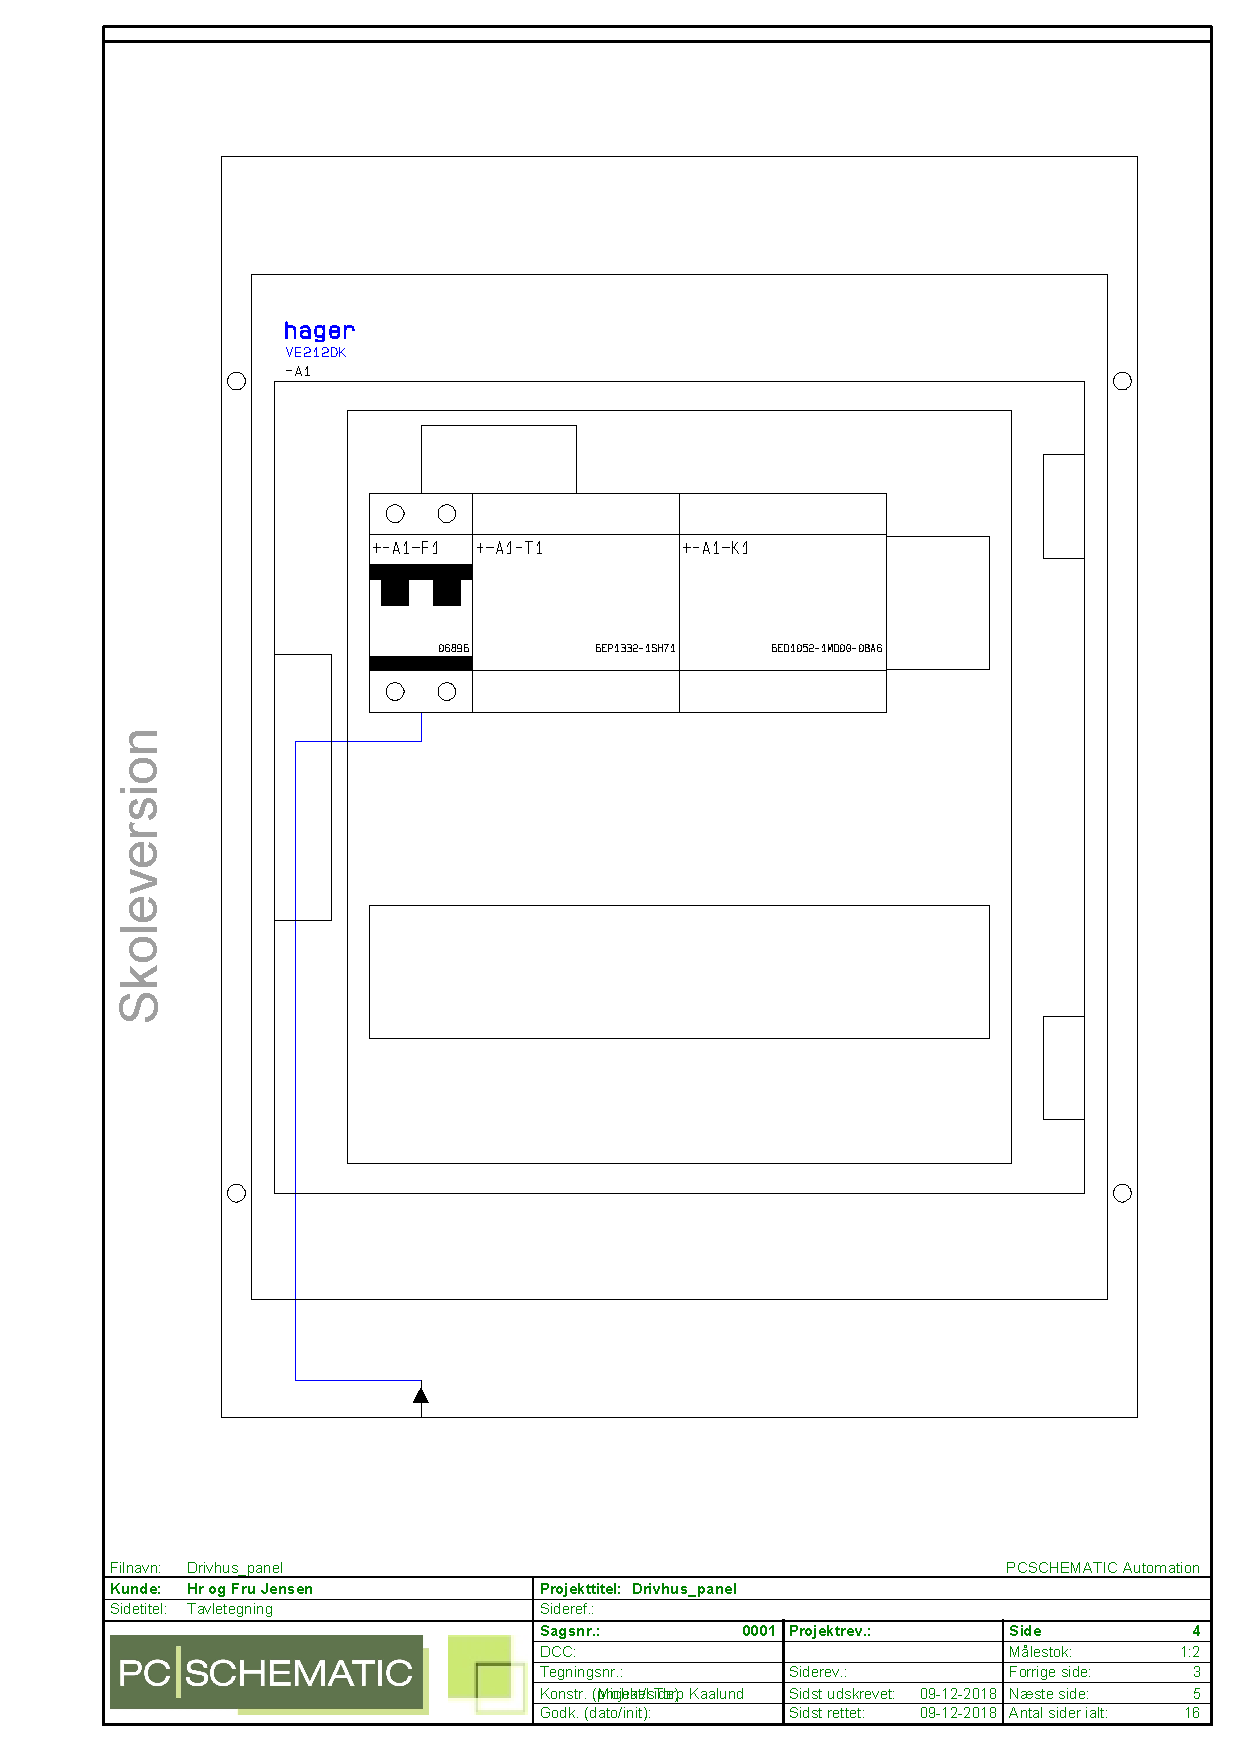
\includegraphics[scale=0.72]{appendix/Drivhus_panel_5.pdf}
\newpage
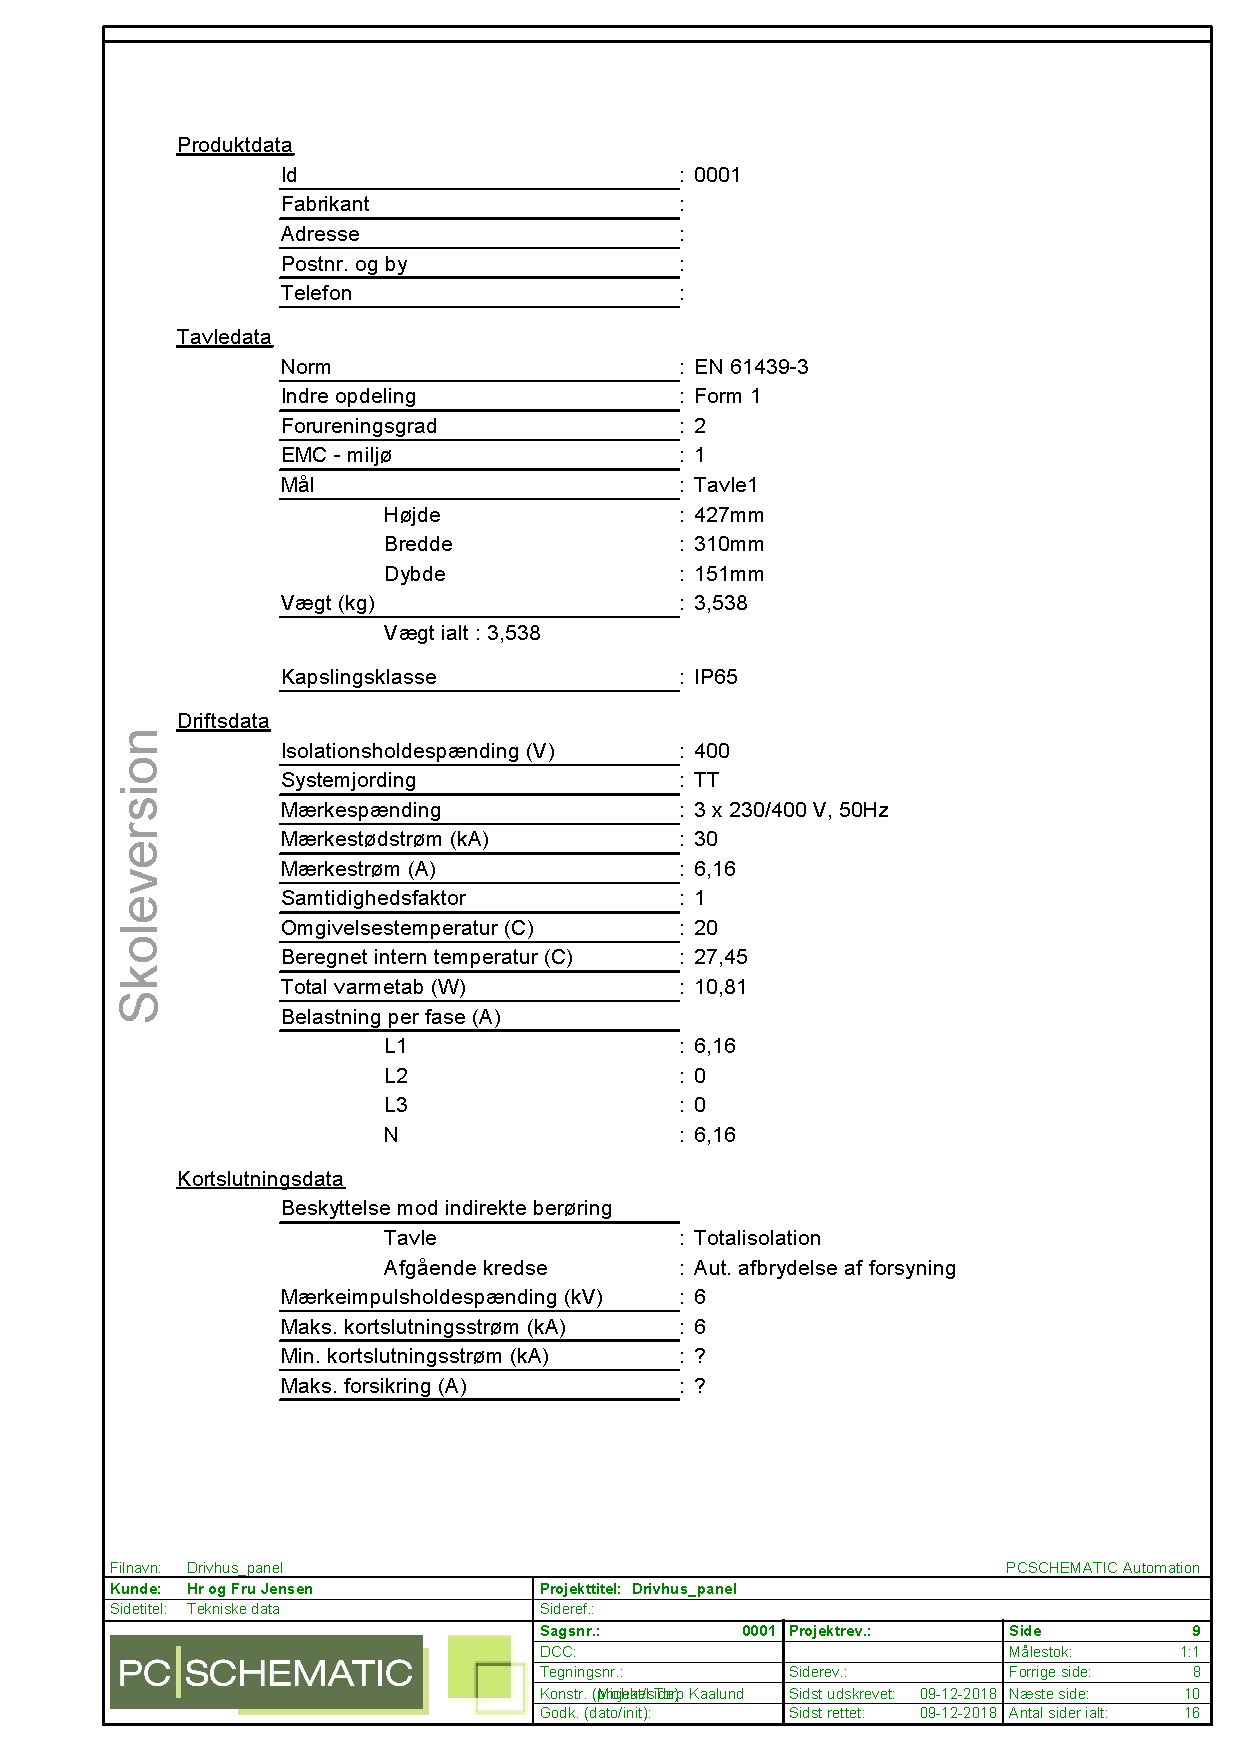
\includegraphics[scale=0.72]{appendix/Drivhus_panel_12.pdf}
\newpage
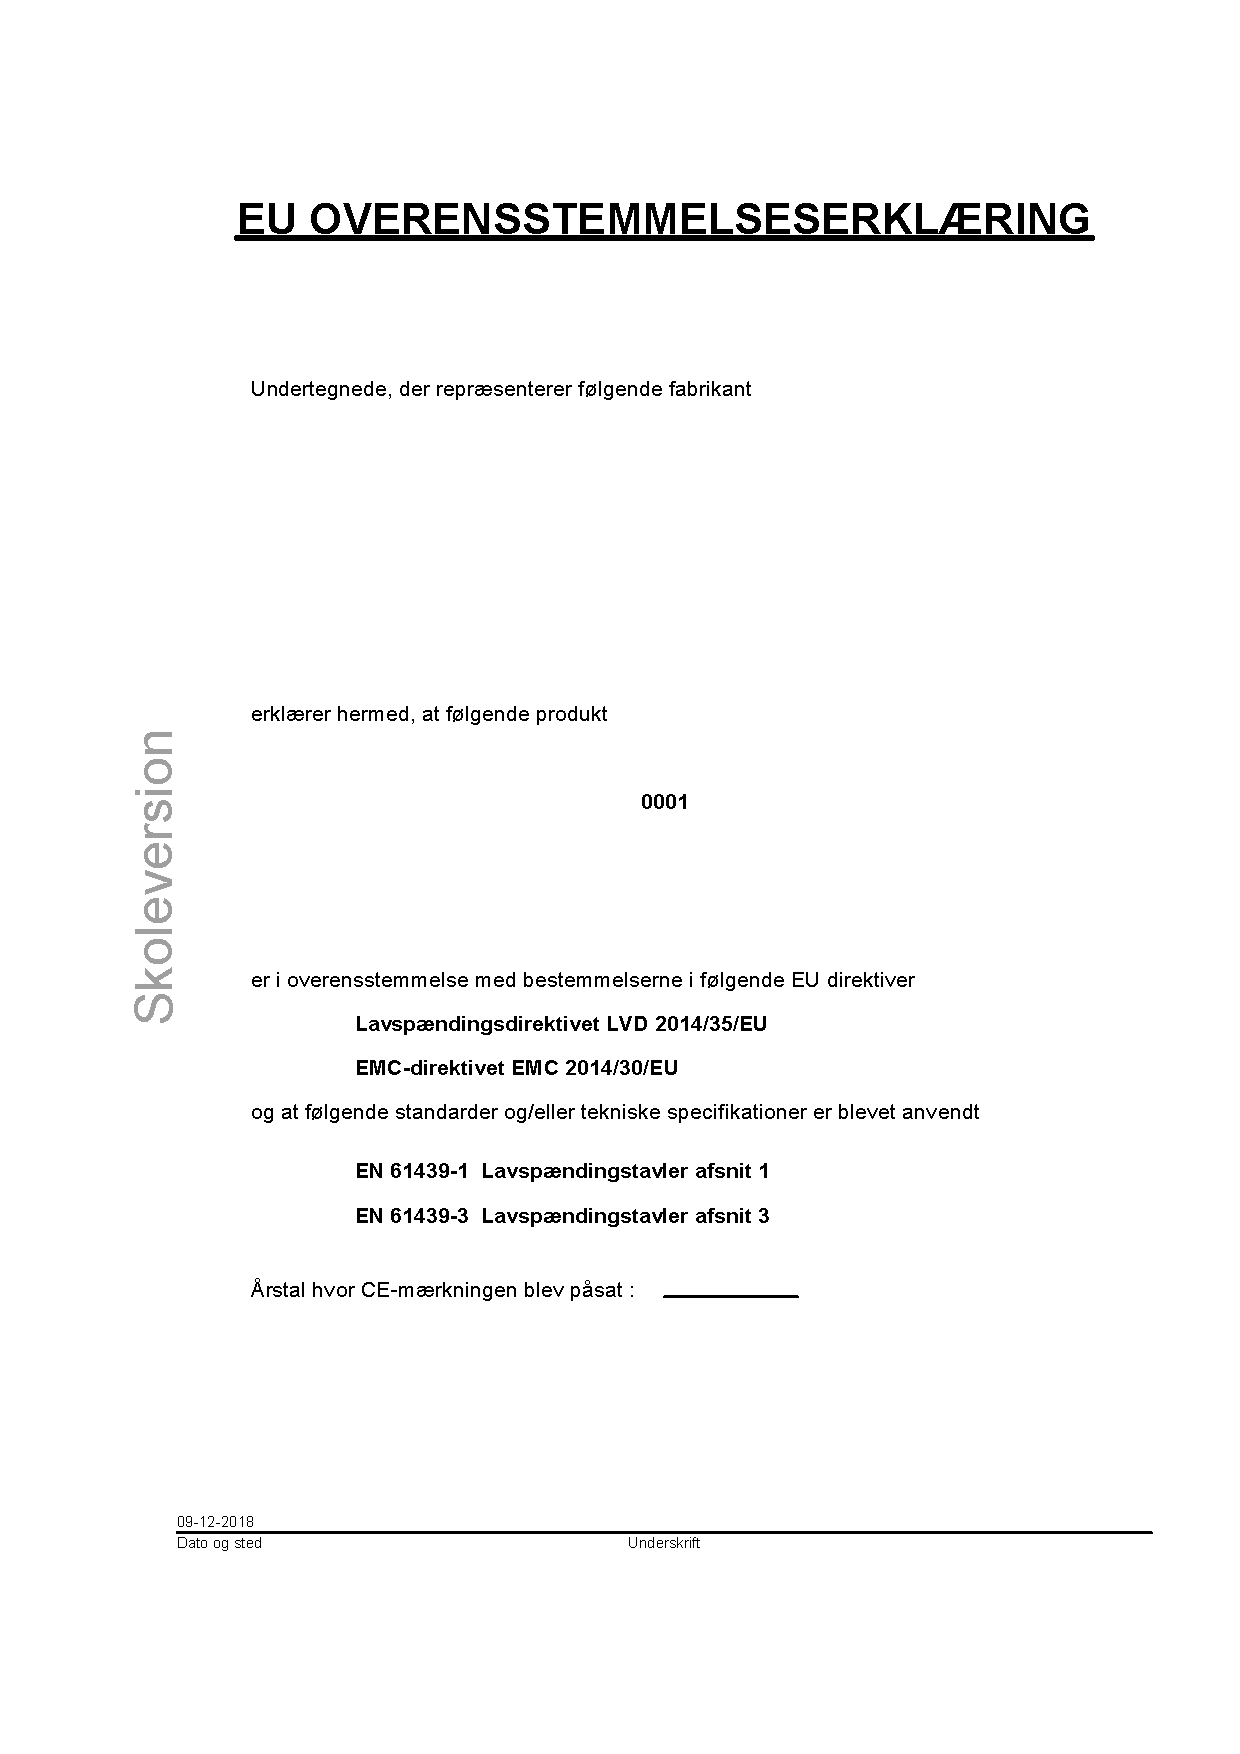
\includegraphics[scale=0.72]{appendix/Drivhus_panel_13.pdf}
%\section{Siemens LOGO! Software}
%\newpage 
%\begin{figure}[!htp]
    %\centering
\subsubsection{Funktionsblokke}
\includegraphics[scale=0.72,angle=90,origin=c]{../LOGO_Program/drivhus_styring_1.pdf}
%\end{figure}
%\newpage
%\begin{figure}[!htp]
    %\centering
\subsubsection{Parameter}
\includegraphics[scale=0.72]{../LOGO_Program/drivhus_styring_2.pdf}
%\end{figure}
\newpage
%\begin{figure}[!htp]
    %\centering
\includegraphics[scale=0.72]{../LOGO_Program/drivhus_styring_3.pdf}
%\end{figure}
%\newpage
%\begin{figure}[!htp]
    %\centering
%\subsection{Kabel forbindelse}
%\includegraphics[scale=0.78]{../LOGO_Program/drivhus_styring_4.pdf}
%\end{figure}
%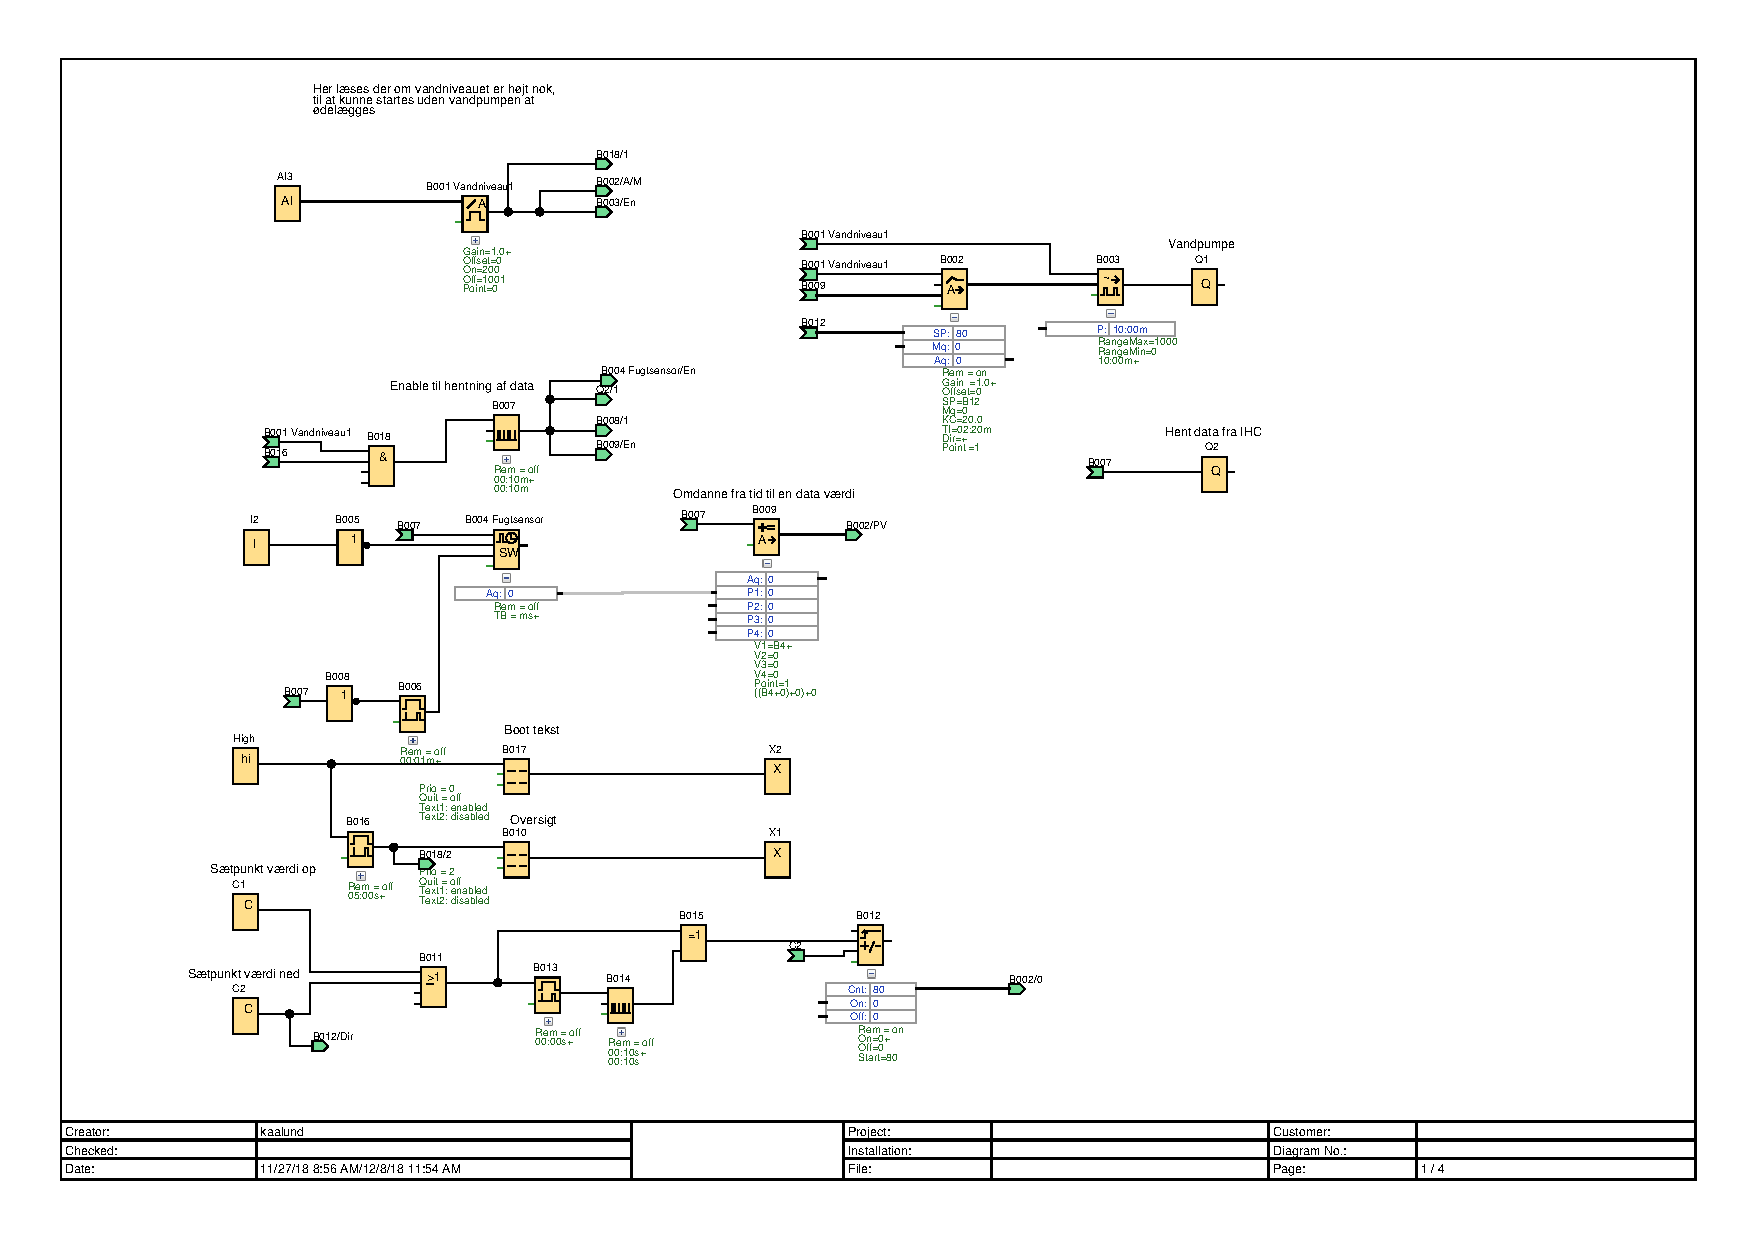
\includepdf[pages=-]{../LOGO_Program/Drivhus_program.pdf}
    \subsection{Ventilation} \label{sub:ventilation}
Der tages udgangspunkt i BR18 [\cite{BR18:Online}] kravene.
Under \S443 står kravene beskrevet at der skal være en udelufttilførsel på mindst 0,3 l/s pr. m$^2$.
I \S443 stk. 3 står der at udsugningen i køkkener skal forøges til mindst 20 l/s og \S443 stk. 4 beskriver udsugningen fra bade- og wc-rum skal kunne forøges til mindst 15 l/s.
Desuden beskreves der også at wc-rum uden bad og bryggers skal der kunne udsuges mindst 10 l/s. 
I forhold til BR15 så der ikke nogle ændring i kravene som har betydning for beregningen.
Dog beskriver BR18, i \S444 at kælder i enfamileshus skal der udsuges mindst 10 l/s.

\subsubsection{Bestemmelse af minimumskravet til anlægget} \label{subsub:minimumkrav_ventilation}
Da kravene for lufttilførelsen kun gælder for de opvarmet beboelse kvm,
det betyder at ydre vægge ikke behøves at være med i udregningen.
I BR18 [\cite{BR18:Online}], 
så skal udelufttilførsel minimum være med 0,3 l/s pr. m$^2$ opvarmet etageareal.
For at kunne lave beregningen, så skal det udregnes til en volumenstrømmen som er i m$^3$/t. 
Dette gøres med at gange 3,6 $\frac{ \text{m}^3 \text{/ l} }{\text{ t / s} }$ for at omregne fra sekunder til timer og liter til kubicmeter.
i tabel \ref{table:samregn_vent_ind} på side \pageref{table:samregn_vent_ind} har jeg regnet ud fra rummenes kvm.

\begin{table}[!h]
     \begin{center}
        \begin{tabular}{|l|r|r|r|}
            \hline
            Rum & kvm & Udelufttilførsel i l/s & Udelufttilførsel i m$^3$/t \\
            \hline
            Soveværelse       & 12,6 m$^2$ & 3,78 l/s & 13,61 m$^3$/t\\
            Stue / Alrum / Køkken & 39,7 m$^2$ & 11,91 l/s & 42,88 m$^3$/t\\
            Entré / Bryggers  & 9,6 m$^2$ & 2,88 l/s & 10,37 m$^3$/t\\
            Gang              & 2,3 m$^2$ & 0,69 l/s & 2,48 m$^3$/t\\
            Værelse 1         & 11,9 m$^2$ & 3,57 l/s & 12,85 m$^3$/t\\
            Værelse 2         & 12,0 m$^2$ & 3,60 l/s & 12,96 m$^3$/t\\
            Bad 1             & 4,3 m$^2$ & 1,29 l/s & 4,64 m$^3$/t\\
            Bad 2             & 7,5 m$^2$ & 2,29 l/s & 8,24 m$^3$/t\\
            \hline
            \hline
            Samlet & \underline{99,9 m$^2$} & \underline{30,01 l/s} & \underline{108,03 m$^3$/t} \\
            \hline
        \end{tabular}
    \end{center}
    \caption{Udregning af Udelufttilførelsens minimumskrav}
    \label{table:samregn_vent_ind}
\end{table}

Så vores krav til udelufttilførsel er at anlægget skal kunne minimum lave et luftskifte på 30,01 l/s.
I BR18 [\cite{BR18:Online}] beskreves der også hvor meget luft som skal udsuges i udvalgte rum, 
de tal skal ligges sammen og ud fra det kan laves en sammenregning til minimumskravet. De udregning findes i tabel \ref{table:samregn_vent_ud} på side \pageref{table:samregn_vent_ud}.
\begin{table}[!h]
    \begin{center}
       \begin{tabular}{|l|r|r|}
           \hline
           Rum & Udsugning i l/s & Udsugning i m$^3$/t \\
           \hline
           Stue / Alrum / Køkken & 20 l/s & 72 m$^3$/t\\
           Entré / Bryggers  & 15 l/s & 54 m$^3$/t\\
           Bad 1             & 15 l/s & 54 m$^3$/t\\
           Bad 2             & 15 l/s & 54 m$^3$/t\\
           \hline
           \hline
           Samlet & \underline{65 l/s} & \underline{234 m$^3$/t} \\
           \hline
       \end{tabular}
   \end{center}
   \caption{Udregning af udsugnings minimumskrav}
   \label{table:samregn_vent_ud}
\end{table}
Her kan det ses, at minimumskrav til udsugning er højere end til udelufttilførselen. 
Da der ønskes, at der er en ligevægt i ens ventilationssystem så beregnes rør diameteren udfra minimum volumenstrømmen i udsugningen.
\begin{equation}\label{eqn:udregning_rd}
d_{n} = \sqrt{ \frac{q_{v} \cdot 4}{V\cdot\pi\cdot3600}}
\end{equation}
Ligning (\ref{eqn:udregning_rd}) på side \pageref{eqn:udregning_rd} bruges til, udregne diameteren i meter, $V$ er lufthastigheden i $m/s$ og $q_v$ er volumenstrømmen i $m^{3}/t$.
Typisk er lufthastigheden mellem 4 - 10 m/s. 
\begin{align} \label{eqn:udregning_min_rd} 
    d_{n}       &= \sqrt{ \frac{q_{v} \cdot 4}{V\cdot\pi\cdot3600}} = \sqrt{ \frac{234 \cdot 4}{4\cdot\pi\cdot3600}} = 0,1438 m = 143,8 mm
\end{align}
Beregningen af rørdiameteren i ligning (\ref{eqn:udregning_min_rd}) på side \pageref{eqn:udregning_min_rd} er fundet til 143,8 mm, 
ikke findes i lindab's sortiment så vælges rørdiameteren til 160mm.

\subsubsection{Tryktab i udsugning} \label{subsub:tryktab_udsugning}
Der er en oversigts tegning over ventilationssystem på side \pageref{fig:tegning_ventr}. 
Længderne er skrevet på tabel \ref{table:oversigt_l_udsugning} på side \pageref{table:oversigt_l_udsugning}, 
der er også valgt at inkludere hvilket volumenstrømmen som skal være i de enkelte rør. 
\begin{align} \label{eqn:volumenstroem_sammenregning} 
    q_{v}(E) &= q_{v}(F) + q_{v}(H) = 54 + 54 = 108 \text{ m}^3\text{/t}
\end{align}
Alle volumenstrømmene skal omregnes til lufthastighed, 
for at kunne finde frem til tryk tabet i rørene, 
det gøres i ligningen \ref{eqn:omregning_vs_til_lh}.
\begin{align} \label{eqn:omregning_vs_til_lh}
    d_{n} &= \sqrt{ \frac{ q_v \cdot 4 }{ V\cdot \pi \cdot 3600 } }  \nonumber \\
          &\Downarrow  \nonumber \\
    d_{n}^{2} &= \frac{ q_v \cdot 4 }{ V\cdot \pi \cdot 3600 } \nonumber \\
          &\Downarrow \nonumber \\
    V     &= \frac{ q_v \cdot 4 }{ d_{n}^{2} \cdot \pi \cdot 3600 } 
\end{align}
Ved at bruge formulen i \ref{eqn:omregning_vs_til_lh}, 
giver den lufthastighed som bruges til, 
at finde tryktabet per meter i databladet for røret.
\begin{table}[h!]
    \begin{center}
       \begin{tabular}{|l|r|r|r|r|r|}
           \hline
           Længde & meter & q$_{v}$ & V & P$_{a}$ / m & Tryktab\\
           \hline
           A & 1,38 m & 270 m$^3$/t & 3,73 m/s & 1,2 P$_{a}$/m & 1,656 Pa\\
           B & 0,27 m & 162 m$^3$/t & 2,24 m/s & 0,5 P$_{a}$/m & 0,135 Pa\\
           C & 0,75 m & 72  m$^3$/t & 0,99 m/s & 0,1 P$_{a}$/m & 0,075 Pa\\
           D & 4,43 m & 54  m$^3$/t & 0,75 m/s & 0,1 P$_{a}$/m & 0,443 Pa\\
           E & 0,46 m & 108 m$^3$/t & 1,49 m/s & 0,2 P$_{a}$/m  & 0,092 Pa\\
           F & 0,94 m & 54 m$^3$/t & 0,75 m/s & 0,1 P$_{a}$/m & 0,094 Pa\\
           G & 2,79 m & 54 m$^3$/t & 0,75 m/s & 0,1 P$_{a}$/m & 0,279 Pa\\
           H & 0,45 m & 54 m$^3$/t & 0,75 m/s& 0,1 P$_{a}$/m & 0,045 Pa\\
           \hline
       \end{tabular}
   \end{center}
   \caption{Oversigt over længderne brugt i udsugningen}
   \label{table:oversigt_l_udsugning}
\end{table}
I tabel \ref{table:oversigt_l_udsugning}, er lufthastigheden som skal bruges til at finde tryktabet i T-rørene.
Dette gøres ved, at aflæse graferne i databladet for T-stykkerne.
\begin{table}[h!]
    \begin{center}
       \begin{tabular}{|l|r|r|r|}
           \hline
           T-rør & V$_{1}$ & V$_{2}$ & Tryktab \\
           \hline
           T$_{\text{B->A}}$ & 2,24 m/s & 3,73 m/s & 4,8 Pa \\ 
           T$_{\text{C->A}}$ & 0,99 m/s & 3,73 m/s & 2,8 Pa \\
           T$_{\text{E->B}}$ & 1,49 m/s & 2,24 m/s & 0,6 Pa \\
           T$_{\text{D->B}}$ & 0,75 m/s & 2,24 m/s & 1,5 Pa \\
           T$_{\text{F->E}}$ & 0,75 m/s & 1,49 m/s & 0,8 Pa \\
           T$_{\text{G->E}}$ & 0,75 m/s & 1,49 m/s & 1,0 Pa \\
           \hline
       \end{tabular}
   \end{center}
   \caption{Oversigt tryktabet i T-rør}
   \label{table:oversigt_tryktab_t-roer}
\end{table}
Nu kan tryktabet findes på det stykke som er længes væk fra ventilationsanlægget, 
som er rum bad 2.
\begin{table}[h!]
    \begin{center}
       \begin{tabular}{lcr}
           \hline
           \hline
           \textbf{Bad 2} &  & \\
           \hline
           \hline
           Ventil (-5mm åbning) & : & 21,000 Pa \\
           90$^\circ$ BU    & : & 0,500 Pa \\
           Rør$_{\text{H}}$ & : & 0,045 Pa \\
           90$^\circ$ BU    & : & 0,500 Pa \\
           Rør$_{\text{G}}$ & : & 0,279 Pa \\
           T-Stykke$_{\text{G->E}}$  & : & 1,000 Pa\\
           Rør$_{\text{E}}$ & : & 0,092 Pa \\
           T-Stykke$_{\text{E->B}}$  & : & 0,600 Pa\\
           Rør$_{\text{B}}$ & : & 0,135 Pa \\
           T-Stykke$_{\text{B->A}}$  & : & 4,800 Pa\\
           Rør$_{\text{A}}$ & : & 1,656 Pa \\
           \hline
           Samlet tryktab    & : & \underline{\underline{ 30,607 Pa}} 
       \end{tabular}
   \end{center}
   %\caption{Oversigt tryktabet i T-rør}
   %\label{table:oversigt_tryktab_t-roer}
\end{table}

\subsubsection{Tryktab i indblæsning} \label{subsub:tryktab_indblaesning}
I tabel \ref{table:oversigt_l_indblaesning}, beskriver længderne brugt til indblæsningen. 
Lufthastighed, Tryktab per meter beskrevet i tabellen er fundet ved hjælp af lindab's App `Vent Tools',
og tryktabet er herefter udregnet fra de tal.
\begin{table}[h!]
    \begin{center}
       \begin{tabular}{|l|r|r|r|r|r|}
           \hline
           Længde & meter & q$_{v}$ & V & P$_{a}$ / m & Tryktab\\
           \hline
            P & 3,94 m & 13,61 m$^3$/t & 0,19 m/s & 0,0 P$_{a}$/m & 0 Pa\\
            O & 0,74 m & 13,61 m$^3$/t & 0,19 m/s & 0,0 P$_{a}$/m & 0 Pa\\
            N & 4,71 m & 56,49 m$^3$/t & 0,78 m/s & 0,1 P$_{a}$/m & 0,471 Pa\\
            M & 4,24 m & 12,96 m$^3$/t & 0,18 m/s & 0,0 P$_{a}$/m & 0 Pa\\
            K & 3,50 m & 25,81 m$^3$/t & 0,36 m/s & 0,0 P$_{a}$/m & 0 Pa\\
            J & 1,78 m & 82,30 m$^3$/t & 1,14 m/s & 0,1 P$_{a}$/m & 0,178 Pa\\
            I & 0,74 m & 82,30 m$^3$/t & 1,14 m/s & 0,1 P$_{a}$/m & 0,074 Pa\\
           \hline
       \end{tabular}
   \end{center}
   \caption{Oversigt over længderne brugt i indblæsning}
   \label{table:oversigt_l_indblaesning}
\end{table}
Tryktabet i T-stykkerne er beskrevet i tabel \ref{table:oversigt_tryktab_t-roer_ind}. 
Lufthastighed for Stue/Alrum/Køkken og Værelse 1 er beregnet ud fra \ref{eqn:omregning_vs_til_lh} på side \pageref{eqn:omregning_vs_til_lh}.
Stue's udregning kan se i udregning \ref{eqn:udregning_af_vs_stue}.
\begin{align} \label{eqn:udregning_af_vs_stue}
    V     &= \frac{ q_v \cdot 4 }{ d_{n}^{2} \cdot \pi \cdot 3600 } \nonumber \\
    V     &= \frac{ 42,88 \cdot 4 }{ (160/1000)^{2} \cdot \pi \cdot 3600 } \nonumber \\
    V     &= \frac{ 171,53 }{ 92,16 \cdot \pi } \nonumber \\
    V     &= 0,592 \text{ m/s}
\end{align}
Når der aflæses i databladet for T-stykkerne, så er det udenfor skalaen.
Det kommer af, at rørdiameteren er sat efter udsugning det sætter lufthastigheden ned og derfor kan tabet sættes til 0 Pa.
Det betyder, at indblæsningen ikke ville have noget tab af betydning i T-stykkerne.
\begin{table}[h!]
    \begin{center}
       \begin{tabular}{|l|r|r|r|}
           \hline
           T-rør & V$_{1}$ & V$_{2}$ & Tryktab \\
           \hline
           T$_{\text{J->N}}$ & 1,14 m/s & 0,78 m/s & 0 Pa \\ 
           T$_{\text{J->K}}$ & 1,14 m/s & 0,36 m/s & 0 Pa \\ 
           T$_{\text{N->O}}$ & 0,78 m/s & 0,19 m/s & 0 Pa \\ 
           T$_{\text{N->Stue}}$ & 0,78 m/s & 0,59 m/s & 0 Pa \\ 
           T$_{\text{K->M}}$ & 0,36 m/s & 0,18 m/s & 0 Pa \\ 
           T$_{\text{K->Værelse 1}}$ & 0,36 m/s & 0,71 m/s & 0 Pa \\ 
           \hline
       \end{tabular}
   \end{center}
   \caption{Oversigt tryktabet i T-rør for indblæsning}
   \label{table:oversigt_tryktab_t-roer_ind}
\end{table}
Nu kan tabet findes på den længeste strækning. Som er på indblæsning er soveværelset.
\begin{table}[h!]
    \begin{center}
       \begin{tabular}{lcr}
           \hline
           \hline
           \textbf{Soveværelse} &  & \\
           \hline
           \hline
           Ventil (6mm åbning) & : & 15,000 Pa \\
           90$^\circ$ BU    & : & 0 Pa \\
           Rør$_{\text{P}}$ & : & 0 Pa \\
           90$^\circ$ BU    & : & 0 Pa \\
           Rør$_{\text{O}}$ & : & 0 Pa \\
           T-Stykke$_{\text{N->O}}$  & : & 0 Pa\\
           Rør$_{\text{N}}$ & : & 0,471 Pa \\
           T-Stykke$_{\text{J->N}}$  & : & 0 Pa\\
           Rør$_{\text{J}}$ & : & 0,178 Pa \\
           90$^\circ$ BU    & : & 3,800 Pa \\
           Rør$_{\text{I}}$ & : & 0,074 Pa \\
           \hline
           Samlet tryktab & : & \underline{\underline{ 19,523 Pa}} 
       \end{tabular}
   \end{center}
   %\caption{Oversigt tryktabet i T-rør}
   %\label{table:oversigt_tryktab_t-roer}
\end{table}

\subsubsection{Valg af ventilationsaggregater}
\todo{Valgt Beskrive hvordan der skal vælgees}
    \section{IHC tavle}
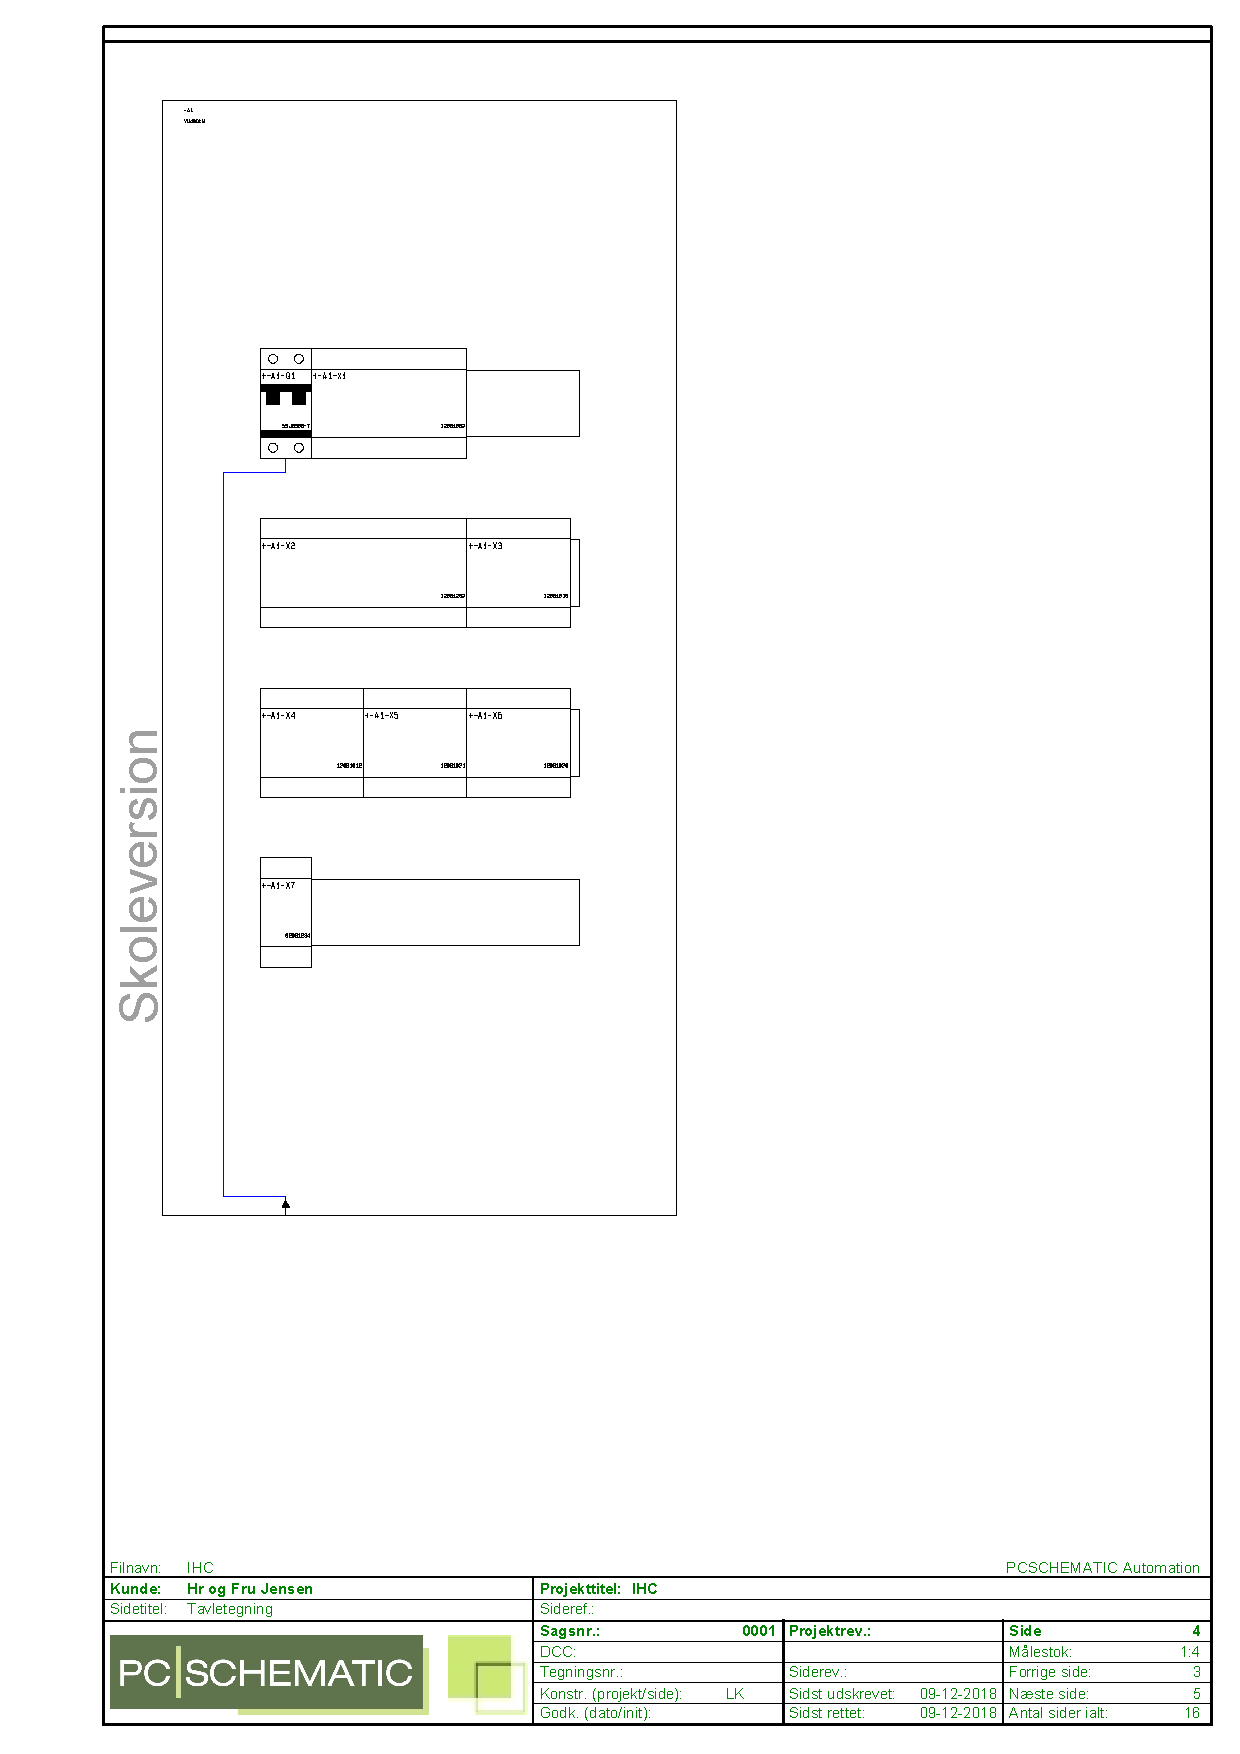
\includegraphics[scale=0.72]{appendix/IHC_side_5.pdf}
\newpage
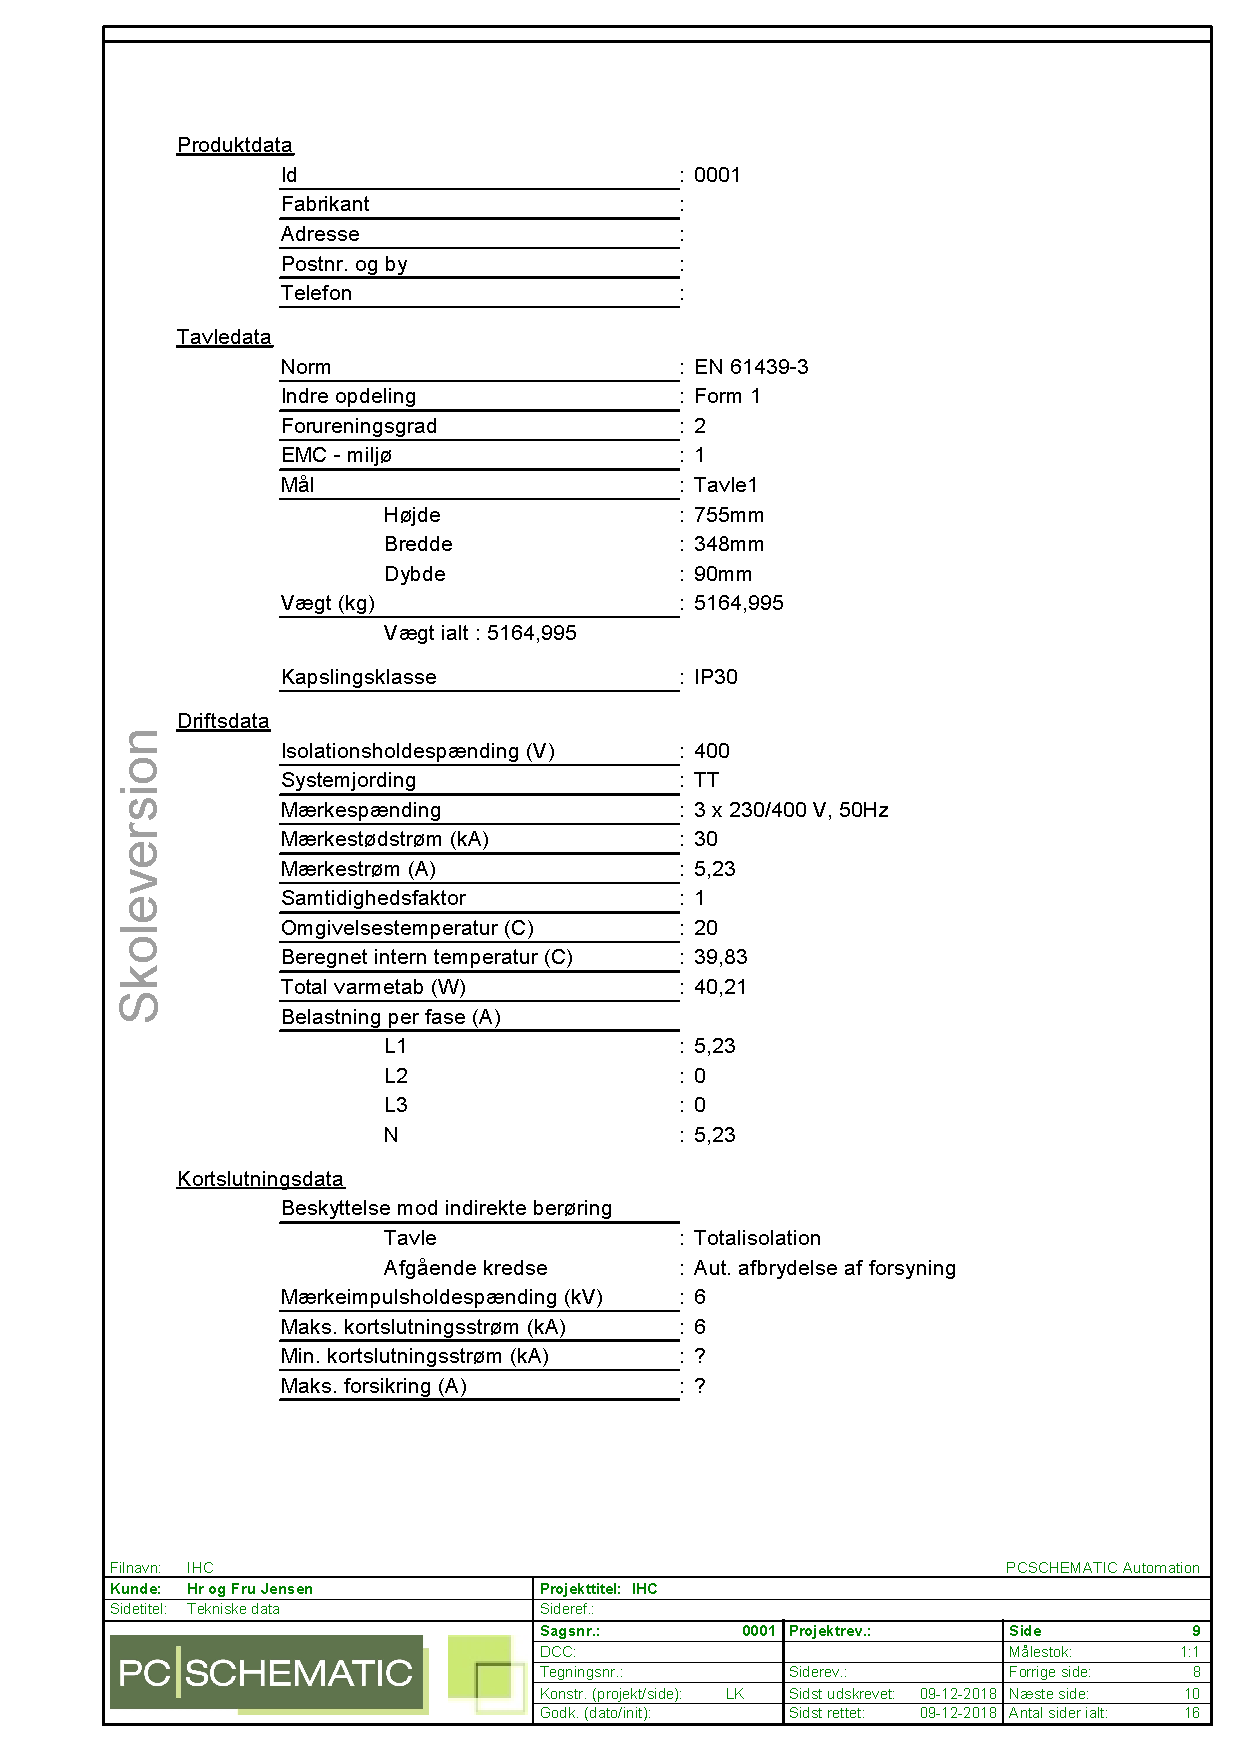
\includegraphics[scale=0.72]{appendix/IHC_side_12.pdf}
\newpage
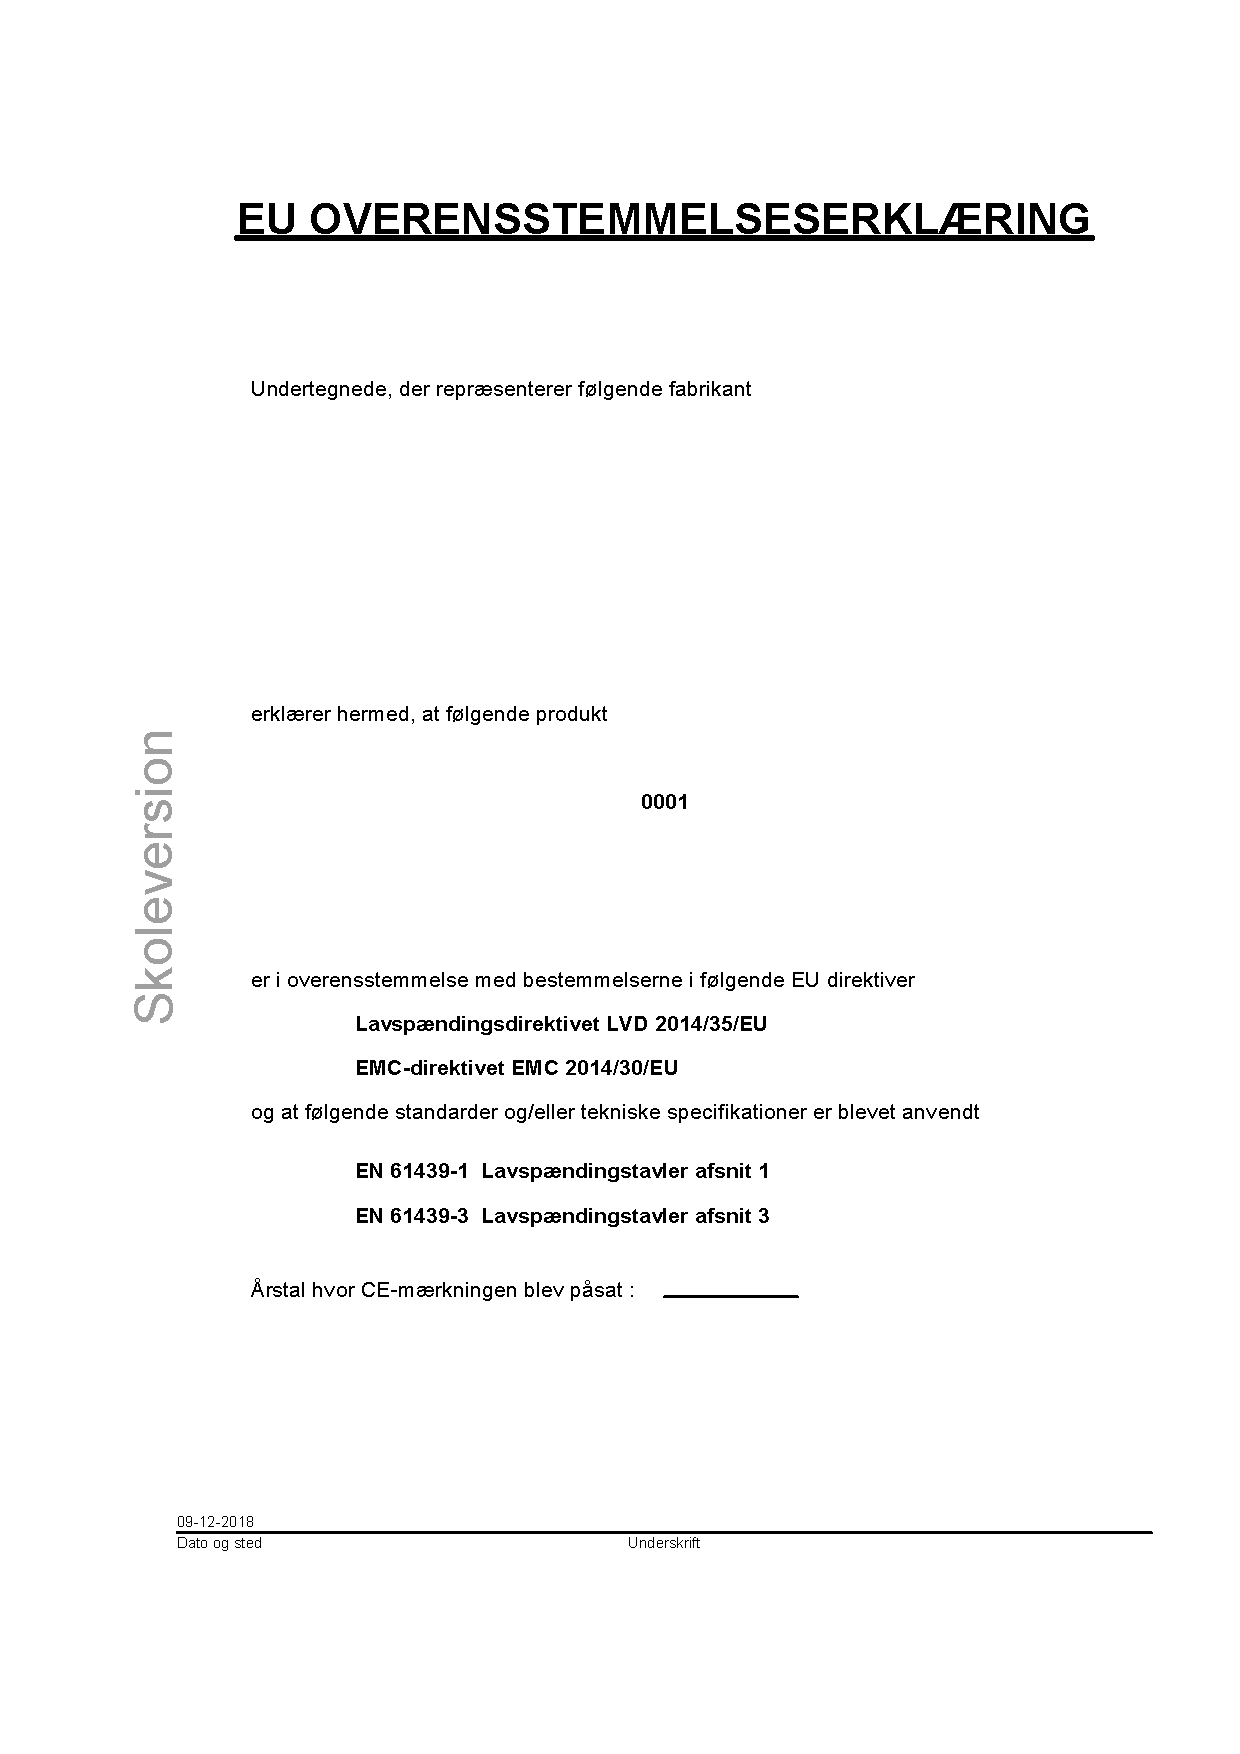
\includegraphics[scale=0.72]{appendix/IHC_side_13.pdf}
    %\section{Home-Assistant}

\subsection{Installationen af Home-Assistant på Raspberry Pi 3 model B+}
Der er en god guide på \url{https://www.home-assistant.io/getting-started/} som anbefales, at følge.
Men den er dog på engelske. Jeg har valgt, at lave en kort beskrivelse af installationen på dansk.
\\
\\
Der er to måder, at installere home-assistant på den ene er at installere den på en eksisterende raspbian billedefil og den anden er at hente en forud konfigueret hass.io billedfil.
Jeg har dog kun valgt, at beskrive installationen af hass.io til Raspberry Pi 3 model B+, da den anden metode er for advanceret bruger af Raspberry Pi og linux styresystemet.


\subsection{Opsætning}
\subsection{Scener}
    %% Program list
    \section{Programmer brug}
\begin{itemize}
    \item Visual Studio Code Version 1.29.1
    \item Siemens LOGO! Soft Comfort Version 8.2
    \item Graphvix
    \item Tex Live 2017
\end{itemize}
    %% Litteratur listen
    %\addcontentsline{toc}{section}{Referancer}
%    \bibliographystyle{plainnat}
    %\bibliographystyle{unsrt} 
    %\bibliography{biblio}
\end{document}